\documentclass[11pt]{article}

    \usepackage[breakable]{tcolorbox}
    \usepackage{parskip} % Stop auto-indenting (to mimic markdown behaviour)
    

    % Basic figure setup, for now with no caption control since it's done
    % automatically by Pandoc (which extracts ![](path) syntax from Markdown).
    \usepackage{graphicx}
    % Keep aspect ratio if custom image width or height is specified
    \setkeys{Gin}{keepaspectratio}
    % Maintain compatibility with old templates. Remove in nbconvert 6.0
    \let\Oldincludegraphics\includegraphics
    % Ensure that by default, figures have no caption (until we provide a
    % proper Figure object with a Caption API and a way to capture that
    % in the conversion process - todo).
    \usepackage{caption}
    \DeclareCaptionFormat{nocaption}{}
    \captionsetup{format=nocaption,aboveskip=0pt,belowskip=0pt}

    \usepackage{float}
    \floatplacement{figure}{H} % forces figures to be placed at the correct location
    \usepackage{xcolor} % Allow colors to be defined
    \usepackage{enumerate} % Needed for markdown enumerations to work
    \usepackage{geometry} % Used to adjust the document margins
    \usepackage{amsmath} % Equations
    \usepackage{amssymb} % Equations
    \usepackage{textcomp} % defines textquotesingle
    % Hack from http://tex.stackexchange.com/a/47451/13684:
    \AtBeginDocument{%
        \def\PYZsq{\textquotesingle}% Upright quotes in Pygmentized code
    }
    \usepackage{upquote} % Upright quotes for verbatim code
    \usepackage{eurosym} % defines \euro

    \usepackage{iftex}
    \ifPDFTeX
        \usepackage[T1]{fontenc}
        \IfFileExists{alphabeta.sty}{
              \usepackage{alphabeta}
          }{
              \usepackage[mathletters]{ucs}
              \usepackage[utf8x]{inputenc}
          }
    \else
        \usepackage{fontspec}
        \usepackage{unicode-math}
    \fi

    \usepackage{fancyvrb} % verbatim replacement that allows latex
    \usepackage{grffile} % extends the file name processing of package graphics
                         % to support a larger range
    \makeatletter % fix for old versions of grffile with XeLaTeX
    \@ifpackagelater{grffile}{2019/11/01}
    {
      % Do nothing on new versions
    }
    {
      \def\Gread@@xetex#1{%
        \IfFileExists{"\Gin@base".bb}%
        {\Gread@eps{\Gin@base.bb}}%
        {\Gread@@xetex@aux#1}%
      }
    }
    \makeatother
    \usepackage[Export]{adjustbox} % Used to constrain images to a maximum size
    \adjustboxset{max size={0.9\linewidth}{0.9\paperheight}}

    % The hyperref package gives us a pdf with properly built
    % internal navigation ('pdf bookmarks' for the table of contents,
    % internal cross-reference links, web links for URLs, etc.)
    \usepackage{hyperref}
    % The default LaTeX title has an obnoxious amount of whitespace. By default,
    % titling removes some of it. It also provides customization options.
    \usepackage{titling}
    \usepackage{longtable} % longtable support required by pandoc >1.10
    \usepackage{booktabs}  % table support for pandoc > 1.12.2
    \usepackage{array}     % table support for pandoc >= 2.11.3
    \usepackage{calc}      % table minipage width calculation for pandoc >= 2.11.1
    \usepackage[inline]{enumitem} % IRkernel/repr support (it uses the enumerate* environment)
    \usepackage[normalem]{ulem} % ulem is needed to support strikethroughs (\sout)
                                % normalem makes italics be italics, not underlines
    \usepackage{soul}      % strikethrough (\st) support for pandoc >= 3.0.0
    \usepackage{mathrsfs}
    

    
    % Colors for the hyperref package
    \definecolor{urlcolor}{rgb}{0,.145,.698}
    \definecolor{linkcolor}{rgb}{.71,0.21,0.01}
    \definecolor{citecolor}{rgb}{.12,.54,.11}

    % ANSI colors
    \definecolor{ansi-black}{HTML}{3E424D}
    \definecolor{ansi-black-intense}{HTML}{282C36}
    \definecolor{ansi-red}{HTML}{E75C58}
    \definecolor{ansi-red-intense}{HTML}{B22B31}
    \definecolor{ansi-green}{HTML}{00A250}
    \definecolor{ansi-green-intense}{HTML}{007427}
    \definecolor{ansi-yellow}{HTML}{DDB62B}
    \definecolor{ansi-yellow-intense}{HTML}{B27D12}
    \definecolor{ansi-blue}{HTML}{208FFB}
    \definecolor{ansi-blue-intense}{HTML}{0065CA}
    \definecolor{ansi-magenta}{HTML}{D160C4}
    \definecolor{ansi-magenta-intense}{HTML}{A03196}
    \definecolor{ansi-cyan}{HTML}{60C6C8}
    \definecolor{ansi-cyan-intense}{HTML}{258F8F}
    \definecolor{ansi-white}{HTML}{C5C1B4}
    \definecolor{ansi-white-intense}{HTML}{A1A6B2}
    \definecolor{ansi-default-inverse-fg}{HTML}{FFFFFF}
    \definecolor{ansi-default-inverse-bg}{HTML}{000000}

    % common color for the border for error outputs.
    \definecolor{outerrorbackground}{HTML}{FFDFDF}

    % commands and environments needed by pandoc snippets
    % extracted from the output of `pandoc -s`
    \providecommand{\tightlist}{%
      \setlength{\itemsep}{0pt}\setlength{\parskip}{0pt}}
    \DefineVerbatimEnvironment{Highlighting}{Verbatim}{commandchars=\\\{\}}
    % Add ',fontsize=\small' for more characters per line
    \newenvironment{Shaded}{}{}
    \newcommand{\KeywordTok}[1]{\textcolor[rgb]{0.00,0.44,0.13}{\textbf{{#1}}}}
    \newcommand{\DataTypeTok}[1]{\textcolor[rgb]{0.56,0.13,0.00}{{#1}}}
    \newcommand{\DecValTok}[1]{\textcolor[rgb]{0.25,0.63,0.44}{{#1}}}
    \newcommand{\BaseNTok}[1]{\textcolor[rgb]{0.25,0.63,0.44}{{#1}}}
    \newcommand{\FloatTok}[1]{\textcolor[rgb]{0.25,0.63,0.44}{{#1}}}
    \newcommand{\CharTok}[1]{\textcolor[rgb]{0.25,0.44,0.63}{{#1}}}
    \newcommand{\StringTok}[1]{\textcolor[rgb]{0.25,0.44,0.63}{{#1}}}
    \newcommand{\CommentTok}[1]{\textcolor[rgb]{0.38,0.63,0.69}{\textit{{#1}}}}
    \newcommand{\OtherTok}[1]{\textcolor[rgb]{0.00,0.44,0.13}{{#1}}}
    \newcommand{\AlertTok}[1]{\textcolor[rgb]{1.00,0.00,0.00}{\textbf{{#1}}}}
    \newcommand{\FunctionTok}[1]{\textcolor[rgb]{0.02,0.16,0.49}{{#1}}}
    \newcommand{\RegionMarkerTok}[1]{{#1}}
    \newcommand{\ErrorTok}[1]{\textcolor[rgb]{1.00,0.00,0.00}{\textbf{{#1}}}}
    \newcommand{\NormalTok}[1]{{#1}}

    % Additional commands for more recent versions of Pandoc
    \newcommand{\ConstantTok}[1]{\textcolor[rgb]{0.53,0.00,0.00}{{#1}}}
    \newcommand{\SpecialCharTok}[1]{\textcolor[rgb]{0.25,0.44,0.63}{{#1}}}
    \newcommand{\VerbatimStringTok}[1]{\textcolor[rgb]{0.25,0.44,0.63}{{#1}}}
    \newcommand{\SpecialStringTok}[1]{\textcolor[rgb]{0.73,0.40,0.53}{{#1}}}
    \newcommand{\ImportTok}[1]{{#1}}
    \newcommand{\DocumentationTok}[1]{\textcolor[rgb]{0.73,0.13,0.13}{\textit{{#1}}}}
    \newcommand{\AnnotationTok}[1]{\textcolor[rgb]{0.38,0.63,0.69}{\textbf{\textit{{#1}}}}}
    \newcommand{\CommentVarTok}[1]{\textcolor[rgb]{0.38,0.63,0.69}{\textbf{\textit{{#1}}}}}
    \newcommand{\VariableTok}[1]{\textcolor[rgb]{0.10,0.09,0.49}{{#1}}}
    \newcommand{\ControlFlowTok}[1]{\textcolor[rgb]{0.00,0.44,0.13}{\textbf{{#1}}}}
    \newcommand{\OperatorTok}[1]{\textcolor[rgb]{0.40,0.40,0.40}{{#1}}}
    \newcommand{\BuiltInTok}[1]{{#1}}
    \newcommand{\ExtensionTok}[1]{{#1}}
    \newcommand{\PreprocessorTok}[1]{\textcolor[rgb]{0.74,0.48,0.00}{{#1}}}
    \newcommand{\AttributeTok}[1]{\textcolor[rgb]{0.49,0.56,0.16}{{#1}}}
    \newcommand{\InformationTok}[1]{\textcolor[rgb]{0.38,0.63,0.69}{\textbf{\textit{{#1}}}}}
    \newcommand{\WarningTok}[1]{\textcolor[rgb]{0.38,0.63,0.69}{\textbf{\textit{{#1}}}}}


    % Define a nice break command that doesn't care if a line doesn't already
    % exist.
    \def\br{\hspace*{\fill} \\* }
    % Math Jax compatibility definitions
    \def\gt{>}
    \def\lt{<}
    \let\Oldtex\TeX
    \let\Oldlatex\LaTeX
    \renewcommand{\TeX}{\textrm{\Oldtex}}
    \renewcommand{\LaTeX}{\textrm{\Oldlatex}}
    % Document parameters
    % Document title
    \title{AML\_LAB\_ASSIGNMENT - 02-1}
    
    
    
    
    
    
    
% Pygments definitions
\makeatletter
\def\PY@reset{\let\PY@it=\relax \let\PY@bf=\relax%
    \let\PY@ul=\relax \let\PY@tc=\relax%
    \let\PY@bc=\relax \let\PY@ff=\relax}
\def\PY@tok#1{\csname PY@tok@#1\endcsname}
\def\PY@toks#1+{\ifx\relax#1\empty\else%
    \PY@tok{#1}\expandafter\PY@toks\fi}
\def\PY@do#1{\PY@bc{\PY@tc{\PY@ul{%
    \PY@it{\PY@bf{\PY@ff{#1}}}}}}}
\def\PY#1#2{\PY@reset\PY@toks#1+\relax+\PY@do{#2}}

\@namedef{PY@tok@w}{\def\PY@tc##1{\textcolor[rgb]{0.73,0.73,0.73}{##1}}}
\@namedef{PY@tok@c}{\let\PY@it=\textit\def\PY@tc##1{\textcolor[rgb]{0.24,0.48,0.48}{##1}}}
\@namedef{PY@tok@cp}{\def\PY@tc##1{\textcolor[rgb]{0.61,0.40,0.00}{##1}}}
\@namedef{PY@tok@k}{\let\PY@bf=\textbf\def\PY@tc##1{\textcolor[rgb]{0.00,0.50,0.00}{##1}}}
\@namedef{PY@tok@kp}{\def\PY@tc##1{\textcolor[rgb]{0.00,0.50,0.00}{##1}}}
\@namedef{PY@tok@kt}{\def\PY@tc##1{\textcolor[rgb]{0.69,0.00,0.25}{##1}}}
\@namedef{PY@tok@o}{\def\PY@tc##1{\textcolor[rgb]{0.40,0.40,0.40}{##1}}}
\@namedef{PY@tok@ow}{\let\PY@bf=\textbf\def\PY@tc##1{\textcolor[rgb]{0.67,0.13,1.00}{##1}}}
\@namedef{PY@tok@nb}{\def\PY@tc##1{\textcolor[rgb]{0.00,0.50,0.00}{##1}}}
\@namedef{PY@tok@nf}{\def\PY@tc##1{\textcolor[rgb]{0.00,0.00,1.00}{##1}}}
\@namedef{PY@tok@nc}{\let\PY@bf=\textbf\def\PY@tc##1{\textcolor[rgb]{0.00,0.00,1.00}{##1}}}
\@namedef{PY@tok@nn}{\let\PY@bf=\textbf\def\PY@tc##1{\textcolor[rgb]{0.00,0.00,1.00}{##1}}}
\@namedef{PY@tok@ne}{\let\PY@bf=\textbf\def\PY@tc##1{\textcolor[rgb]{0.80,0.25,0.22}{##1}}}
\@namedef{PY@tok@nv}{\def\PY@tc##1{\textcolor[rgb]{0.10,0.09,0.49}{##1}}}
\@namedef{PY@tok@no}{\def\PY@tc##1{\textcolor[rgb]{0.53,0.00,0.00}{##1}}}
\@namedef{PY@tok@nl}{\def\PY@tc##1{\textcolor[rgb]{0.46,0.46,0.00}{##1}}}
\@namedef{PY@tok@ni}{\let\PY@bf=\textbf\def\PY@tc##1{\textcolor[rgb]{0.44,0.44,0.44}{##1}}}
\@namedef{PY@tok@na}{\def\PY@tc##1{\textcolor[rgb]{0.41,0.47,0.13}{##1}}}
\@namedef{PY@tok@nt}{\let\PY@bf=\textbf\def\PY@tc##1{\textcolor[rgb]{0.00,0.50,0.00}{##1}}}
\@namedef{PY@tok@nd}{\def\PY@tc##1{\textcolor[rgb]{0.67,0.13,1.00}{##1}}}
\@namedef{PY@tok@s}{\def\PY@tc##1{\textcolor[rgb]{0.73,0.13,0.13}{##1}}}
\@namedef{PY@tok@sd}{\let\PY@it=\textit\def\PY@tc##1{\textcolor[rgb]{0.73,0.13,0.13}{##1}}}
\@namedef{PY@tok@si}{\let\PY@bf=\textbf\def\PY@tc##1{\textcolor[rgb]{0.64,0.35,0.47}{##1}}}
\@namedef{PY@tok@se}{\let\PY@bf=\textbf\def\PY@tc##1{\textcolor[rgb]{0.67,0.36,0.12}{##1}}}
\@namedef{PY@tok@sr}{\def\PY@tc##1{\textcolor[rgb]{0.64,0.35,0.47}{##1}}}
\@namedef{PY@tok@ss}{\def\PY@tc##1{\textcolor[rgb]{0.10,0.09,0.49}{##1}}}
\@namedef{PY@tok@sx}{\def\PY@tc##1{\textcolor[rgb]{0.00,0.50,0.00}{##1}}}
\@namedef{PY@tok@m}{\def\PY@tc##1{\textcolor[rgb]{0.40,0.40,0.40}{##1}}}
\@namedef{PY@tok@gh}{\let\PY@bf=\textbf\def\PY@tc##1{\textcolor[rgb]{0.00,0.00,0.50}{##1}}}
\@namedef{PY@tok@gu}{\let\PY@bf=\textbf\def\PY@tc##1{\textcolor[rgb]{0.50,0.00,0.50}{##1}}}
\@namedef{PY@tok@gd}{\def\PY@tc##1{\textcolor[rgb]{0.63,0.00,0.00}{##1}}}
\@namedef{PY@tok@gi}{\def\PY@tc##1{\textcolor[rgb]{0.00,0.52,0.00}{##1}}}
\@namedef{PY@tok@gr}{\def\PY@tc##1{\textcolor[rgb]{0.89,0.00,0.00}{##1}}}
\@namedef{PY@tok@ge}{\let\PY@it=\textit}
\@namedef{PY@tok@gs}{\let\PY@bf=\textbf}
\@namedef{PY@tok@ges}{\let\PY@bf=\textbf\let\PY@it=\textit}
\@namedef{PY@tok@gp}{\let\PY@bf=\textbf\def\PY@tc##1{\textcolor[rgb]{0.00,0.00,0.50}{##1}}}
\@namedef{PY@tok@go}{\def\PY@tc##1{\textcolor[rgb]{0.44,0.44,0.44}{##1}}}
\@namedef{PY@tok@gt}{\def\PY@tc##1{\textcolor[rgb]{0.00,0.27,0.87}{##1}}}
\@namedef{PY@tok@err}{\def\PY@bc##1{{\setlength{\fboxsep}{\string -\fboxrule}\fcolorbox[rgb]{1.00,0.00,0.00}{1,1,1}{\strut ##1}}}}
\@namedef{PY@tok@kc}{\let\PY@bf=\textbf\def\PY@tc##1{\textcolor[rgb]{0.00,0.50,0.00}{##1}}}
\@namedef{PY@tok@kd}{\let\PY@bf=\textbf\def\PY@tc##1{\textcolor[rgb]{0.00,0.50,0.00}{##1}}}
\@namedef{PY@tok@kn}{\let\PY@bf=\textbf\def\PY@tc##1{\textcolor[rgb]{0.00,0.50,0.00}{##1}}}
\@namedef{PY@tok@kr}{\let\PY@bf=\textbf\def\PY@tc##1{\textcolor[rgb]{0.00,0.50,0.00}{##1}}}
\@namedef{PY@tok@bp}{\def\PY@tc##1{\textcolor[rgb]{0.00,0.50,0.00}{##1}}}
\@namedef{PY@tok@fm}{\def\PY@tc##1{\textcolor[rgb]{0.00,0.00,1.00}{##1}}}
\@namedef{PY@tok@vc}{\def\PY@tc##1{\textcolor[rgb]{0.10,0.09,0.49}{##1}}}
\@namedef{PY@tok@vg}{\def\PY@tc##1{\textcolor[rgb]{0.10,0.09,0.49}{##1}}}
\@namedef{PY@tok@vi}{\def\PY@tc##1{\textcolor[rgb]{0.10,0.09,0.49}{##1}}}
\@namedef{PY@tok@vm}{\def\PY@tc##1{\textcolor[rgb]{0.10,0.09,0.49}{##1}}}
\@namedef{PY@tok@sa}{\def\PY@tc##1{\textcolor[rgb]{0.73,0.13,0.13}{##1}}}
\@namedef{PY@tok@sb}{\def\PY@tc##1{\textcolor[rgb]{0.73,0.13,0.13}{##1}}}
\@namedef{PY@tok@sc}{\def\PY@tc##1{\textcolor[rgb]{0.73,0.13,0.13}{##1}}}
\@namedef{PY@tok@dl}{\def\PY@tc##1{\textcolor[rgb]{0.73,0.13,0.13}{##1}}}
\@namedef{PY@tok@s2}{\def\PY@tc##1{\textcolor[rgb]{0.73,0.13,0.13}{##1}}}
\@namedef{PY@tok@sh}{\def\PY@tc##1{\textcolor[rgb]{0.73,0.13,0.13}{##1}}}
\@namedef{PY@tok@s1}{\def\PY@tc##1{\textcolor[rgb]{0.73,0.13,0.13}{##1}}}
\@namedef{PY@tok@mb}{\def\PY@tc##1{\textcolor[rgb]{0.40,0.40,0.40}{##1}}}
\@namedef{PY@tok@mf}{\def\PY@tc##1{\textcolor[rgb]{0.40,0.40,0.40}{##1}}}
\@namedef{PY@tok@mh}{\def\PY@tc##1{\textcolor[rgb]{0.40,0.40,0.40}{##1}}}
\@namedef{PY@tok@mi}{\def\PY@tc##1{\textcolor[rgb]{0.40,0.40,0.40}{##1}}}
\@namedef{PY@tok@il}{\def\PY@tc##1{\textcolor[rgb]{0.40,0.40,0.40}{##1}}}
\@namedef{PY@tok@mo}{\def\PY@tc##1{\textcolor[rgb]{0.40,0.40,0.40}{##1}}}
\@namedef{PY@tok@ch}{\let\PY@it=\textit\def\PY@tc##1{\textcolor[rgb]{0.24,0.48,0.48}{##1}}}
\@namedef{PY@tok@cm}{\let\PY@it=\textit\def\PY@tc##1{\textcolor[rgb]{0.24,0.48,0.48}{##1}}}
\@namedef{PY@tok@cpf}{\let\PY@it=\textit\def\PY@tc##1{\textcolor[rgb]{0.24,0.48,0.48}{##1}}}
\@namedef{PY@tok@c1}{\let\PY@it=\textit\def\PY@tc##1{\textcolor[rgb]{0.24,0.48,0.48}{##1}}}
\@namedef{PY@tok@cs}{\let\PY@it=\textit\def\PY@tc##1{\textcolor[rgb]{0.24,0.48,0.48}{##1}}}

\def\PYZbs{\char`\\}
\def\PYZus{\char`\_}
\def\PYZob{\char`\{}
\def\PYZcb{\char`\}}
\def\PYZca{\char`\^}
\def\PYZam{\char`\&}
\def\PYZlt{\char`\<}
\def\PYZgt{\char`\>}
\def\PYZsh{\char`\#}
\def\PYZpc{\char`\%}
\def\PYZdl{\char`\$}
\def\PYZhy{\char`\-}
\def\PYZsq{\char`\'}
\def\PYZdq{\char`\"}
\def\PYZti{\char`\~}
% for compatibility with earlier versions
\def\PYZat{@}
\def\PYZlb{[}
\def\PYZrb{]}
\makeatother


    % For linebreaks inside Verbatim environment from package fancyvrb.
    \makeatletter
        \newbox\Wrappedcontinuationbox
        \newbox\Wrappedvisiblespacebox
        \newcommand*\Wrappedvisiblespace {\textcolor{red}{\textvisiblespace}}
        \newcommand*\Wrappedcontinuationsymbol {\textcolor{red}{\llap{\tiny$\m@th\hookrightarrow$}}}
        \newcommand*\Wrappedcontinuationindent {3ex }
        \newcommand*\Wrappedafterbreak {\kern\Wrappedcontinuationindent\copy\Wrappedcontinuationbox}
        % Take advantage of the already applied Pygments mark-up to insert
        % potential linebreaks for TeX processing.
        %        {, <, #, %, $, ' and ": go to next line.
        %        _, }, ^, &, >, - and ~: stay at end of broken line.
        % Use of \textquotesingle for straight quote.
        \newcommand*\Wrappedbreaksatspecials {%
            \def\PYGZus{\discretionary{\char`\_}{\Wrappedafterbreak}{\char`\_}}%
            \def\PYGZob{\discretionary{}{\Wrappedafterbreak\char`\{}{\char`\{}}%
            \def\PYGZcb{\discretionary{\char`\}}{\Wrappedafterbreak}{\char`\}}}%
            \def\PYGZca{\discretionary{\char`\^}{\Wrappedafterbreak}{\char`\^}}%
            \def\PYGZam{\discretionary{\char`\&}{\Wrappedafterbreak}{\char`\&}}%
            \def\PYGZlt{\discretionary{}{\Wrappedafterbreak\char`\<}{\char`\<}}%
            \def\PYGZgt{\discretionary{\char`\>}{\Wrappedafterbreak}{\char`\>}}%
            \def\PYGZsh{\discretionary{}{\Wrappedafterbreak\char`\#}{\char`\#}}%
            \def\PYGZpc{\discretionary{}{\Wrappedafterbreak\char`\%}{\char`\%}}%
            \def\PYGZdl{\discretionary{}{\Wrappedafterbreak\char`\$}{\char`\$}}%
            \def\PYGZhy{\discretionary{\char`\-}{\Wrappedafterbreak}{\char`\-}}%
            \def\PYGZsq{\discretionary{}{\Wrappedafterbreak\textquotesingle}{\textquotesingle}}%
            \def\PYGZdq{\discretionary{}{\Wrappedafterbreak\char`\"}{\char`\"}}%
            \def\PYGZti{\discretionary{\char`\~}{\Wrappedafterbreak}{\char`\~}}%
        }
        % Some characters . , ; ? ! / are not pygmentized.
        % This macro makes them "active" and they will insert potential linebreaks
        \newcommand*\Wrappedbreaksatpunct {%
            \lccode`\~`\.\lowercase{\def~}{\discretionary{\hbox{\char`\.}}{\Wrappedafterbreak}{\hbox{\char`\.}}}%
            \lccode`\~`\,\lowercase{\def~}{\discretionary{\hbox{\char`\,}}{\Wrappedafterbreak}{\hbox{\char`\,}}}%
            \lccode`\~`\;\lowercase{\def~}{\discretionary{\hbox{\char`\;}}{\Wrappedafterbreak}{\hbox{\char`\;}}}%
            \lccode`\~`\:\lowercase{\def~}{\discretionary{\hbox{\char`\:}}{\Wrappedafterbreak}{\hbox{\char`\:}}}%
            \lccode`\~`\?\lowercase{\def~}{\discretionary{\hbox{\char`\?}}{\Wrappedafterbreak}{\hbox{\char`\?}}}%
            \lccode`\~`\!\lowercase{\def~}{\discretionary{\hbox{\char`\!}}{\Wrappedafterbreak}{\hbox{\char`\!}}}%
            \lccode`\~`\/\lowercase{\def~}{\discretionary{\hbox{\char`\/}}{\Wrappedafterbreak}{\hbox{\char`\/}}}%
            \catcode`\.\active
            \catcode`\,\active
            \catcode`\;\active
            \catcode`\:\active
            \catcode`\?\active
            \catcode`\!\active
            \catcode`\/\active
            \lccode`\~`\~
        }
    \makeatother

    \let\OriginalVerbatim=\Verbatim
    \makeatletter
    \renewcommand{\Verbatim}[1][1]{%
        %\parskip\z@skip
        \sbox\Wrappedcontinuationbox {\Wrappedcontinuationsymbol}%
        \sbox\Wrappedvisiblespacebox {\FV@SetupFont\Wrappedvisiblespace}%
        \def\FancyVerbFormatLine ##1{\hsize\linewidth
            \vtop{\raggedright\hyphenpenalty\z@\exhyphenpenalty\z@
                \doublehyphendemerits\z@\finalhyphendemerits\z@
                \strut ##1\strut}%
        }%
        % If the linebreak is at a space, the latter will be displayed as visible
        % space at end of first line, and a continuation symbol starts next line.
        % Stretch/shrink are however usually zero for typewriter font.
        \def\FV@Space {%
            \nobreak\hskip\z@ plus\fontdimen3\font minus\fontdimen4\font
            \discretionary{\copy\Wrappedvisiblespacebox}{\Wrappedafterbreak}
            {\kern\fontdimen2\font}%
        }%

        % Allow breaks at special characters using \PYG... macros.
        \Wrappedbreaksatspecials
        % Breaks at punctuation characters . , ; ? ! and / need catcode=\active
        \OriginalVerbatim[#1,codes*=\Wrappedbreaksatpunct]%
    }
    \makeatother

    % Exact colors from NB
    \definecolor{incolor}{HTML}{303F9F}
    \definecolor{outcolor}{HTML}{D84315}
    \definecolor{cellborder}{HTML}{CFCFCF}
    \definecolor{cellbackground}{HTML}{F7F7F7}

    % prompt
    \makeatletter
    \newcommand{\boxspacing}{\kern\kvtcb@left@rule\kern\kvtcb@boxsep}
    \makeatother
    \newcommand{\prompt}[4]{
        {\ttfamily\llap{{\color{#2}[#3]:\hspace{3pt}#4}}\vspace{-\baselineskip}}
    }
    

    
    % Prevent overflowing lines due to hard-to-break entities
    \sloppy
    % Setup hyperref package
    \hypersetup{
      breaklinks=true,  % so long urls are correctly broken across lines
      colorlinks=true,
      urlcolor=urlcolor,
      linkcolor=linkcolor,
      citecolor=citecolor,
      }
    % Slightly bigger margins than the latex defaults
    
    \geometry{verbose,tmargin=1in,bmargin=1in,lmargin=1in,rmargin=1in}
    
    

\begin{document}
    
    \maketitle
    
    

    
    \section{Transformer Architecture Lab
Assignment}\label{transformer-architecture-lab-assignment}

This lab assignment is designed to give you practical experience with
building and understanding the Transformer architecture, as proposed by
Vaswani et al.~in ``Attention is All You Need''. The assignment is
divided into several sections, each focusing on a key component of the
Transformer model. You will implement these components from scratch,
following the TODOs provided.

\subsection{Learning Objectives}\label{learning-objectives}

\begin{itemize}
\tightlist
\item
  Understand the internals of the Transformer architecture.
\item
  Implement the Scaled Dot-Product Attention mechanism.
\item
  Build the Multi-Head Attention mechanism.
\item
  Assemble the Transformer Encoder Block.
\item
  Integrate Positional Encoding.
\end{itemize}

\subsection{Before You Start}\label{before-you-start}

Make sure you have a basic understanding of the following concepts: -
PyTorch or another deep learning framework. - The concept of neural
networks, especially feed-forward and attention mechanisms. - How
gradient backpropagation works.

\subsection{References for Learning}\label{references-for-learning}

\begin{itemize}
\tightlist
\item
  ``Attention is All You Need'', Vaswani et al., 2017 (Original
  Transformer paper).
\item
  \href{http://jalammar.github.io/illustrated-transformer/}{The
  Illustrated Transformer}, Jay Alammar. Provides an excellent visual
  and intuitive understanding of the model.
\item
  \href{https://pytorch.org/tutorials/}{PyTorch Official Tutorials} for
  a refresher on PyTorch.
\end{itemize}

    \subsection{Section 1: Scaled Dot-Product
Attention}\label{section-1-scaled-dot-product-attention}

    Scaled Dot-Product Attention is a fundamental mechanism at the heart of
the Transformer architecture, introduced in the paper ``Attention Is All
You Need'' by Vaswani et al.~This mechanism allows the model to
dynamically focus on different parts of the input sequence when
performing a task, making it very effective for tasks that benefit from
understanding the relationships and relative positioning of tokens in
the sequence, such as language understanding and generation.

\begin{figure}
\centering
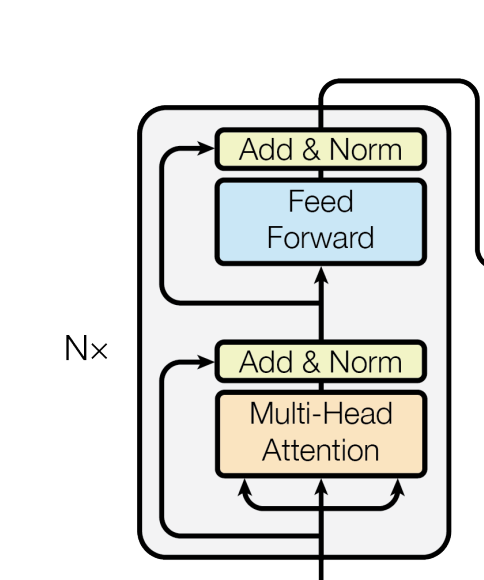
\includegraphics{image.png}
\caption{image.png}
\end{figure}

How It Works The mechanism computes attention scores based on queries
(Q), keys (K), and values (V) derived from the input data, typically
through learned linear transformations. The attention scores determine
how much focus should be placed on each part of the input data when
producing the output for a particular token.

The operation is defined as follows:

\(\text{Attention}(Q,K,V) = \text{softmax}\left( \frac{QK^T}{\sqrt{d_k}} \right)V\)

Q, K, V: These are matrices created from the input embeddings, where Q
represents the queries, K the keys, and V the values. In the context of
self-attention, these are derived from the same input sequence but
transformed differently.

QK\^{}T: This is the dimensionality of the keys (and queries). The
scaling factor \(\sqrt{d_k}\) is used to avoid extremely large values of
the dot product, especially in higher dimensions, which can lead to
vanishing gradients during training. This scaling helps stabilize the
gradient descent optimization process.

Softmax: The softmax function is applied to the rows of the dot product
matrix, turning them into probabilities that sum to 1. This operation
determines how much each value is expressed at a certain position in the
output sequence, effectively allowing the model to focus on relevant
parts of the input.

    \begin{tcolorbox}[breakable, size=fbox, boxrule=1pt, pad at break*=1mm,colback=cellbackground, colframe=cellborder]
\prompt{In}{incolor}{1}{\boxspacing}
\begin{Verbatim}[commandchars=\\\{\}]
\PY{k+kn}{import} \PY{n+nn}{torch}\PY{n+nn}{.}\PY{n+nn}{nn}\PY{n+nn}{.}\PY{n+nn}{functional} \PY{k}{as} \PY{n+nn}{F}
\PY{k+kn}{import} \PY{n+nn}{torch}

\PY{k}{def} \PY{n+nf}{scaled\PYZus{}dot\PYZus{}product}\PY{p}{(}\PY{n}{q}\PY{p}{,} \PY{n}{k}\PY{p}{,} \PY{n}{v}\PY{p}{)}\PY{p}{:}
    \PY{n}{d\PYZus{}k} \PY{o}{=} \PY{n}{q}\PY{o}{.}\PY{n}{size}\PY{p}{(}\PY{o}{\PYZhy{}}\PY{l+m+mi}{1}\PY{p}{)}
    \PY{n}{scores} \PY{o}{=} \PY{n}{torch}\PY{o}{.}\PY{n}{matmul}\PY{p}{(}\PY{n}{q}\PY{p}{,} \PY{n}{k}\PY{o}{.}\PY{n}{transpose}\PY{p}{(}\PY{o}{\PYZhy{}}\PY{l+m+mi}{2}\PY{p}{,} \PY{o}{\PYZhy{}}\PY{l+m+mi}{1}\PY{p}{)}\PY{p}{)} \PY{o}{/} \PY{n}{torch}\PY{o}{.}\PY{n}{sqrt}\PY{p}{(}\PY{n}{torch}\PY{o}{.}\PY{n}{tensor}\PY{p}{(}\PY{n}{d\PYZus{}k}\PY{p}{,} \PY{n}{dtype}\PY{o}{=}\PY{n}{torch}\PY{o}{.}\PY{n}{float32}\PY{p}{)}\PY{p}{)}
    \PY{n}{attention\PYZus{}weights} \PY{o}{=} \PY{n}{F}\PY{o}{.}\PY{n}{softmax}\PY{p}{(}\PY{n}{scores}\PY{p}{,} \PY{n}{dim}\PY{o}{=}\PY{o}{\PYZhy{}}\PY{l+m+mi}{1}\PY{p}{)}
    \PY{n}{output} \PY{o}{=} \PY{n}{torch}\PY{o}{.}\PY{n}{matmul}\PY{p}{(}\PY{n}{attention\PYZus{}weights}\PY{p}{,} \PY{n}{v}\PY{p}{)}
    \PY{k}{return} \PY{n}{output}\PY{p}{,} \PY{n}{attention\PYZus{}weights}

\PY{c+c1}{\PYZsh{} Initialize the seed and tensors as provided}
\PY{n}{torch}\PY{o}{.}\PY{n}{manual\PYZus{}seed}\PY{p}{(}\PY{l+m+mi}{42}\PY{p}{)}
\PY{n}{seq\PYZus{}len}\PY{p}{,} \PY{n}{d\PYZus{}k} \PY{o}{=} \PY{l+m+mi}{3}\PY{p}{,} \PY{l+m+mi}{2}
\PY{n}{q} \PY{o}{=} \PY{n}{torch}\PY{o}{.}\PY{n}{randn}\PY{p}{(}\PY{n}{seq\PYZus{}len}\PY{p}{,} \PY{n}{d\PYZus{}k}\PY{p}{)}
\PY{n}{k} \PY{o}{=} \PY{n}{torch}\PY{o}{.}\PY{n}{randn}\PY{p}{(}\PY{n}{seq\PYZus{}len}\PY{p}{,} \PY{n}{d\PYZus{}k}\PY{p}{)}
\PY{n}{v} \PY{o}{=} \PY{n}{torch}\PY{o}{.}\PY{n}{randn}\PY{p}{(}\PY{n}{seq\PYZus{}len}\PY{p}{,} \PY{n}{d\PYZus{}k}\PY{p}{)}

\PY{n}{values}\PY{p}{,} \PY{n}{attention} \PY{o}{=} \PY{n}{scaled\PYZus{}dot\PYZus{}product}\PY{p}{(}\PY{n}{q}\PY{p}{,} \PY{n}{k}\PY{p}{,} \PY{n}{v}\PY{p}{)}

\PY{n+nb}{print}\PY{p}{(}\PY{l+s+s2}{\PYZdq{}}\PY{l+s+s2}{Q}\PY{l+s+se}{\PYZbs{}n}\PY{l+s+s2}{\PYZdq{}}\PY{p}{,} \PY{n}{q}\PY{p}{)}
\PY{n+nb}{print}\PY{p}{(}\PY{l+s+s2}{\PYZdq{}}\PY{l+s+s2}{K}\PY{l+s+se}{\PYZbs{}n}\PY{l+s+s2}{\PYZdq{}}\PY{p}{,} \PY{n}{k}\PY{p}{)}
\PY{n+nb}{print}\PY{p}{(}\PY{l+s+s2}{\PYZdq{}}\PY{l+s+s2}{V}\PY{l+s+se}{\PYZbs{}n}\PY{l+s+s2}{\PYZdq{}}\PY{p}{,} \PY{n}{v}\PY{p}{)}
\PY{n+nb}{print}\PY{p}{(}\PY{l+s+s2}{\PYZdq{}}\PY{l+s+s2}{Values}\PY{l+s+se}{\PYZbs{}n}\PY{l+s+s2}{\PYZdq{}}\PY{p}{,} \PY{n}{values}\PY{p}{)}
\PY{n+nb}{print}\PY{p}{(}\PY{l+s+s2}{\PYZdq{}}\PY{l+s+s2}{Attention}\PY{l+s+se}{\PYZbs{}n}\PY{l+s+s2}{\PYZdq{}}\PY{p}{,} \PY{n}{attention}\PY{p}{)}
\end{Verbatim}
\end{tcolorbox}

    \begin{Verbatim}[commandchars=\\\{\}]
Q
 tensor([[ 0.3367,  0.1288],
        [ 0.2345,  0.2303],
        [-1.1229, -0.1863]])
K
 tensor([[ 2.2082, -0.6380],
        [ 0.4617,  0.2674],
        [ 0.5349,  0.8094]])
V
 tensor([[ 1.1103, -1.6898],
        [-0.9890,  0.9580],
        [ 1.3221,  0.8172]])
Values
 tensor([[ 0.5698, -0.1520],
        [ 0.5379, -0.0265],
        [ 0.2246,  0.5556]])
Attention
 tensor([[0.4028, 0.2886, 0.3086],
        [0.3538, 0.3069, 0.3393],
        [0.1303, 0.4630, 0.4067]])
    \end{Verbatim}

    \subsection{Section 2: Multi-Head
Attention}\label{section-2-multi-head-attention}

    Multi-Head Attention is a pivotal innovation introduced in the
Transformer model, aimed at enhancing the model's ability to focus on
different parts of the input sequence for a given task. It operates on
the principle of dividing the attention mechanism into multiple
``heads,'' enabling the model to simultaneously attend to information
from different representation subspaces at different positions. This
parallel attention processing allows the model to capture a more complex
interplay of features within the input.

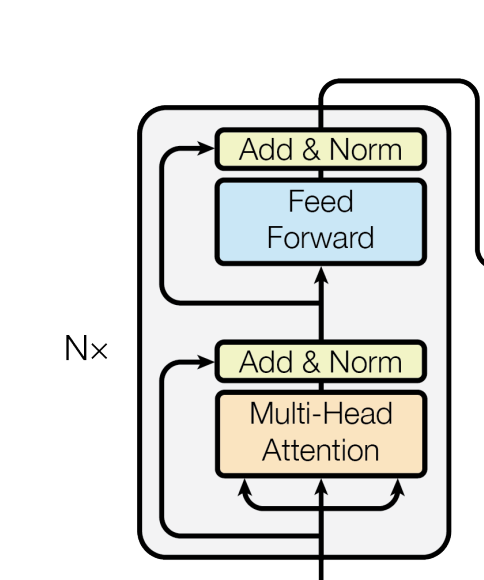
\includegraphics{image.png} \#\# Explanation: Initialization: This class
initializes linear layers for projecting the queries, keys, values, and
the final output. It also calculates d\_k, the dimension of each head.

Splitting Heads: The split\_heads method reshapes the input tensors to
separate heads, allowing the model to process parts of the input in
parallel across different representation subspaces.

Forward Pass: In the forward method, inputs are first projected, then
split into multiple heads. The scaled dot-product attention is computed
for each head. The outputs of all heads are then concatenated and passed
through a final linear projection layer.

This code snippet provides a basic framework for implementing Multi-Head
Attention. In practice, you might need to adjust it based on your
specific requirements, including handling padding masks for
variable-length sequences.

    \begin{tcolorbox}[breakable, size=fbox, boxrule=1pt, pad at break*=1mm,colback=cellbackground, colframe=cellborder]
\prompt{In}{incolor}{2}{\boxspacing}
\begin{Verbatim}[commandchars=\\\{\}]
\PY{k+kn}{import} \PY{n+nn}{torch}
\PY{k+kn}{import} \PY{n+nn}{torch}\PY{n+nn}{.}\PY{n+nn}{nn} \PY{k}{as} \PY{n+nn}{nn}
\PY{k+kn}{import} \PY{n+nn}{torch}\PY{n+nn}{.}\PY{n+nn}{nn}\PY{n+nn}{.}\PY{n+nn}{functional} \PY{k}{as} \PY{n+nn}{F}

\PY{k}{class} \PY{n+nc}{MultiHeadAttention}\PY{p}{(}\PY{n}{nn}\PY{o}{.}\PY{n}{Module}\PY{p}{)}\PY{p}{:}
    \PY{k}{def} \PY{n+nf+fm}{\PYZus{}\PYZus{}init\PYZus{}\PYZus{}}\PY{p}{(}\PY{n+nb+bp}{self}\PY{p}{,} \PY{n}{d\PYZus{}model}\PY{p}{,} \PY{n}{num\PYZus{}heads}\PY{p}{)}\PY{p}{:}
        \PY{n+nb}{super}\PY{p}{(}\PY{n}{MultiHeadAttention}\PY{p}{,} \PY{n+nb+bp}{self}\PY{p}{)}\PY{o}{.}\PY{n+nf+fm}{\PYZus{}\PYZus{}init\PYZus{}\PYZus{}}\PY{p}{(}\PY{p}{)}
        \PY{n+nb+bp}{self}\PY{o}{.}\PY{n}{num\PYZus{}heads} \PY{o}{=} \PY{n}{num\PYZus{}heads}
        \PY{n+nb+bp}{self}\PY{o}{.}\PY{n}{d\PYZus{}model} \PY{o}{=} \PY{n}{d\PYZus{}model}
        \PY{n+nb+bp}{self}\PY{o}{.}\PY{n}{d\PYZus{}k} \PY{o}{=} \PY{n}{d\PYZus{}model} \PY{o}{/}\PY{o}{/} \PY{n}{num\PYZus{}heads}

        \PY{n+nb+bp}{self}\PY{o}{.}\PY{n}{query\PYZus{}projection} \PY{o}{=} \PY{n}{nn}\PY{o}{.}\PY{n}{Linear}\PY{p}{(}\PY{n}{d\PYZus{}model}\PY{p}{,} \PY{n}{d\PYZus{}model}\PY{p}{)}
        \PY{n+nb+bp}{self}\PY{o}{.}\PY{n}{key\PYZus{}projection} \PY{o}{=} \PY{n}{nn}\PY{o}{.}\PY{n}{Linear}\PY{p}{(}\PY{n}{d\PYZus{}model}\PY{p}{,} \PY{n}{d\PYZus{}model}\PY{p}{)}
        \PY{n+nb+bp}{self}\PY{o}{.}\PY{n}{value\PYZus{}projection} \PY{o}{=} \PY{n}{nn}\PY{o}{.}\PY{n}{Linear}\PY{p}{(}\PY{n}{d\PYZus{}model}\PY{p}{,} \PY{n}{d\PYZus{}model}\PY{p}{)}
        \PY{n+nb+bp}{self}\PY{o}{.}\PY{n}{final\PYZus{}projection} \PY{o}{=} \PY{n}{nn}\PY{o}{.}\PY{n}{Linear}\PY{p}{(}\PY{n}{d\PYZus{}model}\PY{p}{,} \PY{n}{d\PYZus{}model}\PY{p}{)}

        \PY{n+nb+bp}{self}\PY{o}{.}\PY{n}{scale} \PY{o}{=} \PY{n}{torch}\PY{o}{.}\PY{n}{sqrt}\PY{p}{(}\PY{n}{torch}\PY{o}{.}\PY{n}{FloatTensor}\PY{p}{(}\PY{p}{[}\PY{n+nb+bp}{self}\PY{o}{.}\PY{n}{d\PYZus{}k}\PY{p}{]}\PY{p}{)}\PY{p}{)}

    \PY{k}{def} \PY{n+nf}{split\PYZus{}heads}\PY{p}{(}\PY{n+nb+bp}{self}\PY{p}{,} \PY{n}{x}\PY{p}{,} \PY{n}{batch\PYZus{}size}\PY{p}{)}\PY{p}{:}
        
        \PY{c+c1}{\PYZsh{}Todo 1.1}
        \PY{c+c1}{\PYZsh{} Split the last dimension into (num\PYZus{}heads, depth)}
        \PY{n}{x} \PY{o}{=} \PY{n}{x}\PY{o}{.}\PY{n}{view}\PY{p}{(}\PY{n}{batch\PYZus{}size}\PY{p}{,}\PY{o}{\PYZhy{}}\PY{l+m+mi}{1}\PY{p}{,}\PY{n+nb+bp}{self}\PY{o}{.}\PY{n}{num\PYZus{}heads}\PY{p}{,}\PY{n+nb+bp}{self}\PY{o}{.}\PY{n}{d\PYZus{}k}\PY{p}{)}
        \PY{c+c1}{\PYZsh{}Todo 1.2}
        \PY{k}{return} \PY{n}{x}\PY{o}{.}\PY{n}{permute}\PY{p}{(}\PY{l+m+mi}{0}\PY{p}{,}\PY{l+m+mi}{2}\PY{p}{,}\PY{l+m+mi}{1}\PY{p}{,}\PY{l+m+mi}{3}\PY{p}{)}  \PY{c+c1}{\PYZsh{} (batch\PYZus{}size, num\PYZus{}heads, seq\PYZus{}length, depth)}

    \PY{k}{def} \PY{n+nf}{forward}\PY{p}{(}\PY{n+nb+bp}{self}\PY{p}{,} \PY{n}{query}\PY{p}{,} \PY{n}{key}\PY{p}{,} \PY{n}{value}\PY{p}{,} \PY{n}{mask}\PY{o}{=}\PY{k+kc}{None}\PY{p}{)}\PY{p}{:}
        \PY{n}{batch\PYZus{}size} \PY{o}{=} \PY{n}{query}\PY{o}{.}\PY{n}{size}\PY{p}{(}\PY{l+m+mi}{0}\PY{p}{)}

        \PY{c+c1}{\PYZsh{} Get query, key and value from responding projection layer}
        \PY{n}{query} \PY{o}{=} \PY{n+nb+bp}{self}\PY{o}{.}\PY{n}{query\PYZus{}projection}\PY{p}{(}\PY{n}{query}\PY{p}{)}
        \PY{n}{key} \PY{o}{=} \PY{n+nb+bp}{self}\PY{o}{.}\PY{n}{key\PYZus{}projection}\PY{p}{(}\PY{n}{key}\PY{p}{)}
        \PY{n}{value} \PY{o}{=} \PY{n+nb+bp}{self}\PY{o}{.}\PY{n}{value\PYZus{}projection}\PY{p}{(}\PY{n}{value}\PY{p}{)}
        
        

        \PY{c+c1}{\PYZsh{} Split query, key and value to multiple heads}
        \PY{c+c1}{\PYZsh{}Todo 1.3}
        \PY{n}{query} \PY{o}{=} \PY{n+nb+bp}{self}\PY{o}{.}\PY{n}{split\PYZus{}heads}\PY{p}{(}\PY{n}{query}\PY{p}{,}\PY{n}{batch\PYZus{}size}\PY{p}{)}
        \PY{n}{key} \PY{o}{=} \PY{n+nb+bp}{self}\PY{o}{.}\PY{n}{split\PYZus{}heads}\PY{p}{(}\PY{n}{key}\PY{p}{,}\PY{n}{batch\PYZus{}size}\PY{p}{)}
        \PY{n}{value} \PY{o}{=} \PY{n+nb+bp}{self}\PY{o}{.}\PY{n}{split\PYZus{}heads}\PY{p}{(}\PY{n}{value}\PY{p}{,}\PY{n}{batch\PYZus{}size}\PY{p}{)}

        \PY{c+c1}{\PYZsh{} Self attention }
        \PY{n}{scores} \PY{o}{=} \PY{n}{torch}\PY{o}{.}\PY{n}{matmul}\PY{p}{(}\PY{n}{query}\PY{p}{,} \PY{n}{key}\PY{o}{.}\PY{n}{transpose}\PY{p}{(}\PY{o}{\PYZhy{}}\PY{l+m+mi}{2}\PY{p}{,} \PY{o}{\PYZhy{}}\PY{l+m+mi}{1}\PY{p}{)}\PY{p}{)} \PY{o}{/} \PY{n+nb+bp}{self}\PY{o}{.}\PY{n}{scale}

        \PY{k}{if} \PY{n}{mask} \PY{o+ow}{is} \PY{o+ow}{not} \PY{k+kc}{None}\PY{p}{:}
            \PY{c+c1}{\PYZsh{} Todo 1.4}
            \PY{c+c1}{\PYZsh{}Sets attention scores to \PYZhy{}inf where mask is 0. This prevents masked elements from influencing the attention output by making them negligible after softmax.}
            \PY{n}{scores} \PY{o}{=} \PY{n}{scores}\PY{o}{.}\PY{n}{masked\PYZus{}fill}\PY{p}{(}\PY{n}{mask} \PY{o}{==} \PY{l+m+mi}{0}\PY{p}{,} \PY{n+nb}{float}\PY{p}{(}\PY{l+s+s1}{\PYZsq{}}\PY{l+s+s1}{\PYZhy{}inf}\PY{l+s+s1}{\PYZsq{}}\PY{p}{)}\PY{p}{)}\PY{c+c1}{\PYZsh{}code here}
            
        \PY{c+c1}{\PYZsh{}Applies softmax to the scores, converting them into a probability distribution that sums to 1, representing the importance of each value.}
        \PY{n}{attention\PYZus{}weights} \PY{o}{=} \PY{n}{F}\PY{o}{.}\PY{n}{softmax}\PY{p}{(}\PY{n}{scores}\PY{p}{,}\PY{n}{dim}\PY{o}{=} \PY{o}{\PYZhy{}}\PY{l+m+mi}{1}\PY{p}{)}
        
        \PY{c+c1}{\PYZsh{}Multiplies attention weights by the value vectors to get the final attention output, effectively selecting or highlighting information based on computed importance.}
        \PY{n}{attention\PYZus{}output} \PY{o}{=} \PY{n}{torch}\PY{o}{.}\PY{n}{matmul}\PY{p}{(}\PY{n}{attention\PYZus{}weights}\PY{p}{,} \PY{n}{value}\PY{p}{)}
        
        \PY{n}{attention\PYZus{}output} \PY{o}{=} \PY{n}{attention\PYZus{}output}\PY{o}{.}\PY{n}{permute}\PY{p}{(}\PY{l+m+mi}{0}\PY{p}{,} \PY{l+m+mi}{2}\PY{p}{,} \PY{l+m+mi}{1}\PY{p}{,} \PY{l+m+mi}{3}\PY{p}{)}\PY{o}{.}\PY{n}{contiguous}\PY{p}{(}\PY{p}{)}

        \PY{c+c1}{\PYZsh{} Concatenate heads}
        \PY{c+c1}{\PYZsh{}Todo 1.5}
        \PY{c+c1}{\PYZsh{} Reshape the attention output tensor to concatenate the heads}

        \PY{n}{attention\PYZus{}output} \PY{o}{=} \PY{n}{attention\PYZus{}output}\PY{o}{.}\PY{n}{view}\PY{p}{(}\PY{n}{batch\PYZus{}size}\PY{p}{,} \PY{o}{\PYZhy{}}\PY{l+m+mi}{1}\PY{p}{,} \PY{n+nb+bp}{self}\PY{o}{.}\PY{n}{d\PYZus{}model}\PY{p}{)}  \PY{c+c1}{\PYZsh{} Concatenate heads}
        
        
        \PY{c+c1}{\PYZsh{} Final projection}
        \PY{c+c1}{\PYZsh{}Todo 1.6}
        \PY{c+c1}{\PYZsh{} Perform the final projection to transform the concatenated tensor}
        \PY{n}{output} \PY{o}{=} \PY{n+nb+bp}{self}\PY{o}{.}\PY{n}{final\PYZus{}projection}\PY{p}{(}\PY{n}{attention\PYZus{}output}\PY{p}{)}

        \PY{k}{return} \PY{n}{output}\PY{p}{,} \PY{n}{attention\PYZus{}weights}
\end{Verbatim}
\end{tcolorbox}

    Test the Multi Head Attention module

    \begin{tcolorbox}[breakable, size=fbox, boxrule=1pt, pad at break*=1mm,colback=cellbackground, colframe=cellborder]
\prompt{In}{incolor}{3}{\boxspacing}
\begin{Verbatim}[commandchars=\\\{\}]
\PY{c+c1}{\PYZsh{} Example instantiation}
\PY{n}{d\PYZus{}model} \PY{o}{=} \PY{l+m+mi}{512}  \PY{c+c1}{\PYZsh{} Embedding size}
\PY{n}{num\PYZus{}heads} \PY{o}{=} \PY{l+m+mi}{8}
\PY{n}{mha} \PY{o}{=} \PY{n}{MultiHeadAttention}\PY{p}{(}\PY{n}{d\PYZus{}model}\PY{p}{,} \PY{n}{num\PYZus{}heads}\PY{p}{)}

\PY{c+c1}{\PYZsh{} inputs}
\PY{n}{seq\PYZus{}length} \PY{o}{=} \PY{l+m+mi}{60}
\PY{n}{batch\PYZus{}size} \PY{o}{=} \PY{l+m+mi}{20}

\PY{c+c1}{\PYZsh{}Todo 1.7}
\PY{c+c1}{\PYZsh{}pass the values batch\PYZus{}size, seq\PYZus{}length, d\PYZus{}model}
\PY{n}{dummy\PYZus{}query} \PY{o}{=} \PY{n}{torch}\PY{o}{.}\PY{n}{rand}\PY{p}{(}\PY{n}{batch\PYZus{}size}\PY{p}{,} \PY{n}{seq\PYZus{}length}\PY{p}{,} \PY{n}{d\PYZus{}model}\PY{p}{)}
\PY{n}{dummy\PYZus{}key} \PY{o}{=} \PY{n}{torch}\PY{o}{.}\PY{n}{rand}\PY{p}{(}\PY{n}{batch\PYZus{}size}\PY{p}{,} \PY{n}{seq\PYZus{}length}\PY{p}{,} \PY{n}{d\PYZus{}model}\PY{p}{)}
\PY{n}{dummy\PYZus{}value} \PY{o}{=} \PY{n}{torch}\PY{o}{.}\PY{n}{rand}\PY{p}{(}\PY{n}{batch\PYZus{}size}\PY{p}{,} \PY{n}{seq\PYZus{}length}\PY{p}{,} \PY{n}{d\PYZus{}model}\PY{p}{)}

\PY{c+c1}{\PYZsh{} Forward pass}
\PY{n}{output}\PY{p}{,} \PY{n}{attention\PYZus{}weights} \PY{o}{=} \PY{n}{mha}\PY{p}{(}\PY{n}{dummy\PYZus{}query}\PY{p}{,} \PY{n}{dummy\PYZus{}key}\PY{p}{,} \PY{n}{dummy\PYZus{}value}\PY{p}{)}
\PY{n+nb}{print}\PY{p}{(}\PY{n}{output}\PY{o}{.}\PY{n}{shape}\PY{p}{)}  \PY{c+c1}{\PYZsh{} Expected shape: (batch\PYZus{}size, seq\PYZus{}length, d\PYZus{}model)}
\PY{n+nb}{print}\PY{p}{(}\PY{n}{attention\PYZus{}weights}\PY{o}{.}\PY{n}{shape}\PY{p}{)}  \PY{c+c1}{\PYZsh{} Shape: (batch\PYZus{}size, num\PYZus{}heads, seq\PYZus{}length, seq\PYZus{}length)}
\end{Verbatim}
\end{tcolorbox}

    \begin{Verbatim}[commandchars=\\\{\}]
torch.Size([20, 60, 512])
torch.Size([20, 8, 60, 60])
    \end{Verbatim}

    \subsection{Section 3: Transformer Encoder
Block}\label{section-3-transformer-encoder-block}

    The Transformer Encoder Block is a core component of the Transformer
architecture, specifically within the encoder part of the model. It is
designed to process the input sequence in a way that captures both the
individual meaning of each token and the context provided by the rest of
the sequence. Each encoder block is composed of several key components
that work together to achieve this goal.

\begin{figure}
\centering
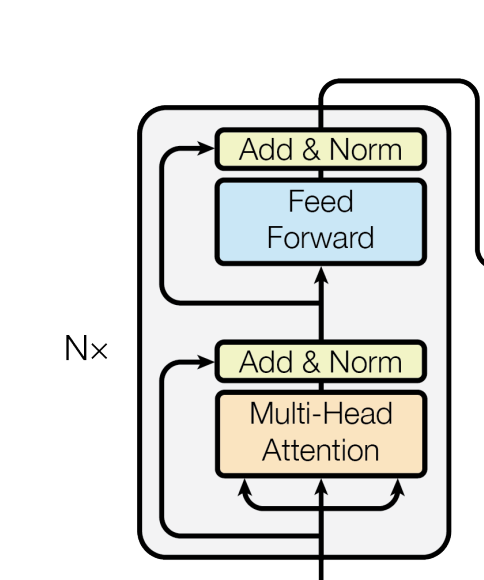
\includegraphics{image.png}
\caption{image.png}
\end{figure}

\subsection{Explanation:}\label{explanation}

Multi-Head Attention: The encoder block starts with a multi-head
attention layer that allows the model to focus on different parts of the
input sequence.

Feedforward Network: After attention, the block applies a position-wise
feedforward network. It's a simple fully connected neural network
applied to each position separately and identically.

Normalization and Dropout: Before and after each of these main layers,
the block applies dropout followed by layer normalization as a form of
regularization and to stabilize the learning process.

Residual Connections: There are residual connections around each of the
main layers (the multi-head attention and the feedforward network). This
helps in mitigating the vanishing gradient problem in deep networks.

This code snippet assumes that the MultiHeadAttention class has been
defined as shown in the previous example. The Transformer Encoder Block
is a fundamental building block of Transformer-based models,
encapsulating the core ideas of multi-head self-attention and
position-wise transformation within a layer normalization and residual
connection framework.

    \begin{tcolorbox}[breakable, size=fbox, boxrule=1pt, pad at break*=1mm,colback=cellbackground, colframe=cellborder]
\prompt{In}{incolor}{4}{\boxspacing}
\begin{Verbatim}[commandchars=\\\{\}]
\PY{k+kn}{import} \PY{n+nn}{torch}
\PY{k+kn}{import} \PY{n+nn}{torch}\PY{n+nn}{.}\PY{n+nn}{nn} \PY{k}{as} \PY{n+nn}{nn}
\PY{k+kn}{import} \PY{n+nn}{torch}\PY{n+nn}{.}\PY{n+nn}{nn}\PY{n+nn}{.}\PY{n+nn}{functional} \PY{k}{as} \PY{n+nn}{F}

\PY{k}{class} \PY{n+nc}{TransformerEncoderBlock}\PY{p}{(}\PY{n}{nn}\PY{o}{.}\PY{n}{Module}\PY{p}{)}\PY{p}{:}
    \PY{k}{def} \PY{n+nf+fm}{\PYZus{}\PYZus{}init\PYZus{}\PYZus{}}\PY{p}{(}\PY{n+nb+bp}{self}\PY{p}{,} \PY{n}{d\PYZus{}model}\PY{p}{,} \PY{n}{num\PYZus{}heads}\PY{p}{,} \PY{n}{d\PYZus{}ff}\PY{p}{,} \PY{n}{dropout\PYZus{}rate}\PY{o}{=}\PY{l+m+mf}{0.1}\PY{p}{)}\PY{p}{:}
        \PY{n+nb}{super}\PY{p}{(}\PY{n}{TransformerEncoderBlock}\PY{p}{,} \PY{n+nb+bp}{self}\PY{p}{)}\PY{o}{.}\PY{n+nf+fm}{\PYZus{}\PYZus{}init\PYZus{}\PYZus{}}\PY{p}{(}\PY{p}{)}
        \PY{n+nb+bp}{self}\PY{o}{.}\PY{n}{multi\PYZus{}head\PYZus{}attention} \PY{o}{=} \PY{n}{MultiHeadAttention}\PY{p}{(}\PY{n}{d\PYZus{}model}\PY{p}{,} \PY{n}{num\PYZus{}heads}\PY{p}{)}

\PY{+w}{        }\PY{l+s+sd}{\PYZdq{}\PYZdq{}\PYZdq{}To do 2.1, implement a feed\PYZus{}forward layer. }
\PY{l+s+sd}{        The architecture is Linear+ReLU+Dropout+Linear}
\PY{l+s+sd}{        \PYZdq{}\PYZdq{}\PYZdq{}}

        \PY{n+nb+bp}{self}\PY{o}{.}\PY{n}{feed\PYZus{}forward} \PY{o}{=} \PY{n}{nn}\PY{o}{.}\PY{n}{Sequential}\PY{p}{(}\PY{n}{nn}\PY{o}{.}\PY{n}{Linear}\PY{p}{(}\PY{n}{d\PYZus{}model}\PY{p}{,} \PY{n}{d\PYZus{}ff}\PY{p}{)}\PY{p}{,}
            \PY{n}{nn}\PY{o}{.}\PY{n}{ReLU}\PY{p}{(}\PY{p}{)}\PY{p}{,}
            \PY{n}{nn}\PY{o}{.}\PY{n}{Dropout}\PY{p}{(}\PY{n}{dropout\PYZus{}rate}\PY{p}{)}\PY{p}{,}
            \PY{n}{nn}\PY{o}{.}\PY{n}{Linear}\PY{p}{(}\PY{n}{d\PYZus{}ff}\PY{p}{,} \PY{n}{d\PYZus{}model}\PY{p}{)}
            
        \PY{p}{)}

        \PY{n+nb+bp}{self}\PY{o}{.}\PY{n}{norm1} \PY{o}{=} \PY{n}{nn}\PY{o}{.}\PY{n}{LayerNorm}\PY{p}{(}\PY{n}{d\PYZus{}model}\PY{p}{)}
        \PY{n+nb+bp}{self}\PY{o}{.}\PY{n}{norm2} \PY{o}{=} \PY{n}{nn}\PY{o}{.}\PY{n}{LayerNorm}\PY{p}{(}\PY{n}{d\PYZus{}model}\PY{p}{)}
        \PY{n+nb+bp}{self}\PY{o}{.}\PY{n}{dropout1} \PY{o}{=} \PY{n}{nn}\PY{o}{.}\PY{n}{Dropout}\PY{p}{(}\PY{n}{dropout\PYZus{}rate}\PY{p}{)}
        \PY{n+nb+bp}{self}\PY{o}{.}\PY{n}{dropout2} \PY{o}{=} \PY{n}{nn}\PY{o}{.}\PY{n}{Dropout}\PY{p}{(}\PY{n}{dropout\PYZus{}rate}\PY{p}{)}

    \PY{k}{def} \PY{n+nf}{forward}\PY{p}{(}\PY{n+nb+bp}{self}\PY{p}{,} \PY{n}{x}\PY{p}{,} \PY{n}{mask}\PY{o}{=}\PY{k+kc}{None}\PY{p}{)}\PY{p}{:}

\PY{+w}{        }\PY{l+s+sd}{\PYZdq{}\PYZdq{}\PYZdq{}To do 2.2: implement the whole forward}
\PY{l+s+sd}{        \PYZdq{}\PYZdq{}\PYZdq{}}
        
        \PY{c+c1}{\PYZsh{} Multi\PYZhy{}Head Attention}
        \PY{n}{attn\PYZus{}output}\PY{p}{,} \PY{n}{\PYZus{}} \PY{o}{=} \PY{n+nb+bp}{self}\PY{o}{.}\PY{n}{multi\PYZus{}head\PYZus{}attention}\PY{p}{(}\PY{n}{x}\PY{p}{,} \PY{n}{x}\PY{p}{,} \PY{n}{x}\PY{p}{,} \PY{n}{mask}\PY{p}{)}
        \PY{n}{x} \PY{o}{=} \PY{n}{x} \PY{o}{+} \PY{n+nb+bp}{self}\PY{o}{.}\PY{n}{dropout1}\PY{p}{(}\PY{n}{attn\PYZus{}output}\PY{p}{)}  \PY{c+c1}{\PYZsh{} Apply dropout to the output of the attention layer}
        \PY{n}{x} \PY{o}{=} \PY{n+nb+bp}{self}\PY{o}{.}\PY{n}{norm1}\PY{p}{(}\PY{n}{x}\PY{p}{)}  \PY{c+c1}{\PYZsh{} Apply LayerNorm}
        
        \PY{c+c1}{\PYZsh{} Feedforward}
        \PY{n}{ff\PYZus{}output} \PY{o}{=} \PY{n+nb+bp}{self}\PY{o}{.}\PY{n}{feed\PYZus{}forward}\PY{p}{(}\PY{n}{x}\PY{p}{)}
        \PY{n}{x} \PY{o}{=} \PY{n}{x} \PY{o}{+} \PY{n+nb+bp}{self}\PY{o}{.}\PY{n}{dropout2}\PY{p}{(}\PY{n}{ff\PYZus{}output}\PY{p}{)}  \PY{c+c1}{\PYZsh{} Apply dropout to the output of the feedforward layer}
        \PY{n}{x} \PY{o}{=} \PY{n+nb+bp}{self}\PY{o}{.}\PY{n}{norm2}\PY{p}{(}\PY{n}{x}\PY{p}{)}  \PY{c+c1}{\PYZsh{} Apply LayerNorm}

        \PY{k}{return} \PY{n}{x}
\end{Verbatim}
\end{tcolorbox}

    Test the Encoderblock module

    \begin{tcolorbox}[breakable, size=fbox, boxrule=1pt, pad at break*=1mm,colback=cellbackground, colframe=cellborder]
\prompt{In}{incolor}{5}{\boxspacing}
\begin{Verbatim}[commandchars=\\\{\}]
\PY{c+c1}{\PYZsh{} Example instantiation}
\PY{n}{d\PYZus{}model} \PY{o}{=} \PY{l+m+mi}{512}  \PY{c+c1}{\PYZsh{} Embedding size}
\PY{n}{num\PYZus{}heads} \PY{o}{=} \PY{l+m+mi}{8}
\PY{n}{d\PYZus{}ff} \PY{o}{=} \PY{l+m+mi}{2048}  \PY{c+c1}{\PYZsh{} Size of the FFN layer}

\PY{c+c1}{\PYZsh{}Todo 3}
\PY{n}{encoder\PYZus{}block} \PY{o}{=} \PY{n}{TransformerEncoderBlock}\PY{p}{(}\PY{n}{d\PYZus{}model}\PY{p}{,} \PY{n}{num\PYZus{}heads}\PY{p}{,} \PY{n}{d\PYZus{}ff}\PY{p}{)}  \PY{c+c1}{\PYZsh{} Instantiate the encoder block}


\PY{c+c1}{\PYZsh{}code here}

\PY{c+c1}{\PYZsh{} input}
\PY{n}{seq\PYZus{}length} \PY{o}{=} \PY{l+m+mi}{60}
\PY{n}{batch\PYZus{}size} \PY{o}{=} \PY{l+m+mi}{20}
\PY{n}{dummy\PYZus{}input} \PY{o}{=} \PY{n}{torch}\PY{o}{.}\PY{n}{rand}\PY{p}{(}\PY{n}{batch\PYZus{}size}\PY{p}{,} \PY{n}{seq\PYZus{}length}\PY{p}{,} \PY{n}{d\PYZus{}model}\PY{p}{)}

\PY{c+c1}{\PYZsh{} Forward pass}
\PY{n}{output} \PY{o}{=} \PY{n}{encoder\PYZus{}block}\PY{p}{(}\PY{n}{dummy\PYZus{}input}\PY{p}{)}
\PY{n+nb}{print}\PY{p}{(}\PY{n}{output}\PY{o}{.}\PY{n}{shape}\PY{p}{)}  \PY{c+c1}{\PYZsh{} Expected shape: (batch\PYZus{}size, seq\PYZus{}length, d\PYZus{}model)}
\end{Verbatim}
\end{tcolorbox}

    \begin{Verbatim}[commandchars=\\\{\}]
torch.Size([20, 60, 512])
    \end{Verbatim}

    \subsection{Section 4: Positional
Encoding}\label{section-4-positional-encoding}

    Positional Encoding is a technique used in the Transformer model to
inject information about the position of each token in the sequence.
Since the Transformer architecture does not inherently process
sequential data in order (unlike RNNs or LSTMs), it lacks a way to
inherently distinguish the order of tokens in the input. Positional
encodings address this limitation by providing a unique signature for
each position that can be added to the token embeddings, thus allowing
the model to take the order of tokens into account.

\begin{split}PE_{(pos,i)} = \begin{cases}
    \sin\left(\frac{pos}{10000^{i/d_{\text{model}}}}\right) & \text{if}\hspace{3mm} i \text{ mod } 2=0\\
    \cos\left(\frac{pos}{10000^{(i-1)/d_{\text{model}}}}\right) & \text{otherwise}\\
\end{cases}\end{split}

\subsection{Explanation:}\label{explanation}

Initialization: The PositionalEncoding module calculates the positional
encodings for positions 0 through max\_len for all dimensions of the
model. The encoding uses a combination of sine and cosine functions of
different frequencies.

Sinusoidal Functions: Odd and even indices of the positional encoding
vector are filled with sine and cosine values, respectively. This
pattern helps the model to distinguish between different positions due
to the unique waveform shapes and frequencies.

Adding to Input Embeddings: The positional encoding is added to the
input embeddings. This ensures that the model can not only learn from
the data but also how the data is positioned relative to each other
within the sequence.

Positional Encoding is essential for the Transformer model to consider
the order of words or elements in the sequence, allowing it to
effectively process sequential data without relying on recurrent layers.

    \begin{tcolorbox}[breakable, size=fbox, boxrule=1pt, pad at break*=1mm,colback=cellbackground, colframe=cellborder]
\prompt{In}{incolor}{6}{\boxspacing}
\begin{Verbatim}[commandchars=\\\{\}]
\PY{k+kn}{import} \PY{n+nn}{torch}
\PY{k+kn}{import} \PY{n+nn}{torch}\PY{n+nn}{.}\PY{n+nn}{nn} \PY{k}{as} \PY{n+nn}{nn}
\PY{k+kn}{import} \PY{n+nn}{numpy} \PY{k}{as} \PY{n+nn}{np}
\PY{k+kn}{import} \PY{n+nn}{matplotlib}\PY{n+nn}{.}\PY{n+nn}{pyplot} \PY{k}{as} \PY{n+nn}{plt}
\PY{k+kn}{import} \PY{n+nn}{math}

\PY{k}{class} \PY{n+nc}{PositionalEncoding}\PY{p}{(}\PY{n}{nn}\PY{o}{.}\PY{n}{Module}\PY{p}{)}\PY{p}{:}
    \PY{k}{def} \PY{n+nf+fm}{\PYZus{}\PYZus{}init\PYZus{}\PYZus{}}\PY{p}{(}\PY{n+nb+bp}{self}\PY{p}{,} \PY{n}{d\PYZus{}model}\PY{p}{,} \PY{n}{max\PYZus{}len}\PY{o}{=}\PY{l+m+mi}{5000}\PY{p}{)}\PY{p}{:}
        \PY{n+nb}{super}\PY{p}{(}\PY{n}{PositionalEncoding}\PY{p}{,} \PY{n+nb+bp}{self}\PY{p}{)}\PY{o}{.}\PY{n+nf+fm}{\PYZus{}\PYZus{}init\PYZus{}\PYZus{}}\PY{p}{(}\PY{p}{)}
\PY{+w}{        }\PY{l+s+sd}{\PYZdq{}\PYZdq{}\PYZdq{}To do: 4.1}
\PY{l+s+sd}{        \PYZdq{}\PYZdq{}\PYZdq{}}
        \PY{c+c1}{\PYZsh{} Generate positions in a sequence up to a maximum length and Add a new dimension to make it a column vector}
        \PY{n}{position} \PY{o}{=} \PY{n}{torch}\PY{o}{.}\PY{n}{arange}\PY{p}{(}\PY{n}{max\PYZus{}len}\PY{p}{)}\PY{o}{.}\PY{n}{unsqueeze}\PY{p}{(}\PY{l+m+mi}{1}\PY{p}{)}
        \PY{c+c1}{\PYZsh{}Calculate the div\PYZus{}term for positional encoding}
        \PY{n}{div\PYZus{}term} \PY{o}{=} \PY{n}{torch}\PY{o}{.}\PY{n}{exp}\PY{p}{(}\PY{n}{torch}\PY{o}{.}\PY{n}{arange}\PY{p}{(}\PY{l+m+mi}{0}\PY{p}{,} \PY{n}{d\PYZus{}model}\PY{p}{,} \PY{l+m+mi}{2}\PY{p}{)}\PY{o}{.}\PY{n}{float}\PY{p}{(}\PY{p}{)} \PY{o}{*} \PY{p}{(}\PY{o}{\PYZhy{}}\PY{n}{math}\PY{o}{.}\PY{n}{log}\PY{p}{(}\PY{l+m+mf}{10000.0}\PY{p}{)} \PY{o}{/} \PY{n}{d\PYZus{}model}\PY{p}{)}\PY{p}{)}
        
        
        
        \PY{n}{pe} \PY{o}{=} \PY{n}{torch}\PY{o}{.}\PY{n}{zeros}\PY{p}{(}\PY{n}{max\PYZus{}len}\PY{p}{,} \PY{n}{d\PYZus{}model}\PY{p}{)}

        \PY{c+c1}{\PYZsh{}Todo 4.2}
        \PY{n}{pe}\PY{p}{[}\PY{p}{:}\PY{p}{,} \PY{l+m+mi}{0}\PY{p}{:}\PY{p}{:}\PY{l+m+mi}{2}\PY{p}{]} \PY{o}{=} \PY{n}{torch}\PY{o}{.}\PY{n}{sin}\PY{p}{(}\PY{n}{position} \PY{o}{*} \PY{n}{div\PYZus{}term}\PY{p}{)}\PY{c+c1}{\PYZsh{} sin function}
        \PY{n}{pe}\PY{p}{[}\PY{p}{:}\PY{p}{,} \PY{l+m+mi}{1}\PY{p}{:}\PY{p}{:}\PY{l+m+mi}{2}\PY{p}{]} \PY{o}{=} \PY{n}{torch}\PY{o}{.}\PY{n}{cos}\PY{p}{(}\PY{n}{position} \PY{o}{*} \PY{n}{div\PYZus{}term}\PY{p}{)}\PY{c+c1}{\PYZsh{} cos function}

        \PY{n}{pe} \PY{o}{=} \PY{n}{pe}\PY{o}{.}\PY{n}{unsqueeze}\PY{p}{(}\PY{l+m+mi}{0}\PY{p}{)}\PY{o}{.}\PY{n}{transpose}\PY{p}{(}\PY{l+m+mi}{0}\PY{p}{,} \PY{l+m+mi}{1}\PY{p}{)}  \PY{c+c1}{\PYZsh{} Shape: [max\PYZus{}len, 1, d\PYZus{}model]}
        \PY{n+nb+bp}{self}\PY{o}{.}\PY{n}{register\PYZus{}buffer}\PY{p}{(}\PY{l+s+s1}{\PYZsq{}}\PY{l+s+s1}{pe}\PY{l+s+s1}{\PYZsq{}}\PY{p}{,} \PY{n}{pe}\PY{p}{)}

    \PY{k}{def} \PY{n+nf}{forward}\PY{p}{(}\PY{n+nb+bp}{self}\PY{p}{,} \PY{n}{x}\PY{p}{)}\PY{p}{:}
        \PY{n}{x} \PY{o}{=} \PY{n}{x} \PY{o}{+} \PY{n+nb+bp}{self}\PY{o}{.}\PY{n}{pe}\PY{p}{[}\PY{p}{:}\PY{n}{x}\PY{o}{.}\PY{n}{size}\PY{p}{(}\PY{l+m+mi}{0}\PY{p}{)}\PY{p}{,} \PY{p}{:}\PY{p}{]}
        \PY{k}{return} \PY{n}{x}
\end{Verbatim}
\end{tcolorbox}

    Test the Positional Encoding function

    \begin{tcolorbox}[breakable, size=fbox, boxrule=1pt, pad at break*=1mm,colback=cellbackground, colframe=cellborder]
\prompt{In}{incolor}{7}{\boxspacing}
\begin{Verbatim}[commandchars=\\\{\}]
\PY{c+c1}{\PYZsh{} Generate the positional encoding for visualization with the definition above}
\PY{n}{d\PYZus{}model} \PY{o}{=} \PY{l+m+mi}{20}  \PY{c+c1}{\PYZsh{} Reduced size for visualization purposes}
\PY{n}{max\PYZus{}len} \PY{o}{=} \PY{l+m+mi}{100}  \PY{c+c1}{\PYZsh{} Sequence length for the visualization}
\PY{n}{pos\PYZus{}encoding} \PY{o}{=} \PY{n}{PositionalEncoding}\PY{p}{(}\PY{n}{d\PYZus{}model}\PY{p}{,} \PY{n}{max\PYZus{}len}\PY{p}{)}
\PY{n}{pos\PYZus{}encoding\PYZus{}matrix} \PY{o}{=} \PY{n}{pos\PYZus{}encoding}\PY{o}{.}\PY{n}{pe}\PY{o}{.}\PY{n}{squeeze}\PY{p}{(}\PY{p}{)}\PY{o}{.}\PY{n}{transpose}\PY{p}{(}\PY{l+m+mi}{0}\PY{p}{,} \PY{l+m+mi}{1}\PY{p}{)}\PY{o}{.}\PY{n}{numpy}\PY{p}{(}\PY{p}{)}

\PY{c+c1}{\PYZsh{} Todo 4.3 Visualizing the positional encoding }
\PY{k+kn}{import} \PY{n+nn}{matplotlib}\PY{n+nn}{.}\PY{n+nn}{pyplot} \PY{k}{as} \PY{n+nn}{plt}  \PY{c+c1}{\PYZsh{} Import matplotlib for visualization}

\PY{c+c1}{\PYZsh{} Visualize the Positional Encoding matrix after ensuring all necessary imports}
\PY{n}{plt}\PY{o}{.}\PY{n}{figure}\PY{p}{(}\PY{n}{figsize}\PY{o}{=}\PY{p}{(}\PY{l+m+mi}{15}\PY{p}{,} \PY{l+m+mi}{10}\PY{p}{)}\PY{p}{)}
\PY{n}{plt}\PY{o}{.}\PY{n}{pcolormesh}\PY{p}{(}\PY{n}{pos\PYZus{}encoding\PYZus{}matrix}\PY{p}{,} \PY{n}{cmap}\PY{o}{=}\PY{l+s+s1}{\PYZsq{}}\PY{l+s+s1}{RdBu}\PY{l+s+s1}{\PYZsq{}}\PY{p}{)}
\PY{n}{plt}\PY{o}{.}\PY{n}{xlabel}\PY{p}{(}\PY{l+s+s1}{\PYZsq{}}\PY{l+s+s1}{Depth}\PY{l+s+s1}{\PYZsq{}}\PY{p}{)}
\PY{n}{plt}\PY{o}{.}\PY{n}{xlim}\PY{p}{(}\PY{p}{(}\PY{l+m+mi}{0}\PY{p}{,} \PY{n}{d\PYZus{}model}\PY{p}{)}\PY{p}{)}
\PY{n}{plt}\PY{o}{.}\PY{n}{ylabel}\PY{p}{(}\PY{l+s+s1}{\PYZsq{}}\PY{l+s+s1}{Position}\PY{l+s+s1}{\PYZsq{}}\PY{p}{)}
\PY{n}{plt}\PY{o}{.}\PY{n}{colorbar}\PY{p}{(}\PY{p}{)}
\PY{n}{plt}\PY{o}{.}\PY{n}{title}\PY{p}{(}\PY{l+s+s1}{\PYZsq{}}\PY{l+s+s1}{Positional Encoding Matrix Heatmap}\PY{l+s+s1}{\PYZsq{}}\PY{p}{)}
\PY{n}{plt}\PY{o}{.}\PY{n}{show}\PY{p}{(}\PY{p}{)}
\end{Verbatim}
\end{tcolorbox}

    \begin{center}
    \adjustimage{max size={0.9\linewidth}{0.9\paperheight}}{output_18_0.png}
    \end{center}
    { \hspace*{\fill} \\}
    
    \section{Marks:}\label{marks}

Todo 1 : 30 Marks

Todo 2 : 35 Marks

Todo 3 : 10 Marks

Todo 4 : 25 Marks

    \begin{tcolorbox}[breakable, size=fbox, boxrule=1pt, pad at break*=1mm,colback=cellbackground, colframe=cellborder]
\prompt{In}{incolor}{8}{\boxspacing}
\begin{Verbatim}[commandchars=\\\{\}]
\PY{n}{pip} \PY{n}{install} \PY{o}{\PYZhy{}}\PY{o}{\PYZhy{}}\PY{n}{upgrade} \PY{n}{nbconvert} \PY{n}{jupyter}
\end{Verbatim}
\end{tcolorbox}

    \begin{Verbatim}[commandchars=\\\{\}]
Requirement already satisfied: nbconvert in
/opt/homebrew/Caskroom/miniconda/base/lib/python3.11/site-packages (7.16.3)
Requirement already satisfied: jupyter in
/opt/homebrew/Caskroom/miniconda/base/lib/python3.11/site-packages (1.0.0)
Requirement already satisfied: beautifulsoup4 in
/opt/homebrew/Caskroom/miniconda/base/lib/python3.11/site-packages (from
nbconvert) (4.12.3)
Requirement already satisfied: bleach!=5.0.0 in
/opt/homebrew/Caskroom/miniconda/base/lib/python3.11/site-packages (from
nbconvert) (6.1.0)
Requirement already satisfied: defusedxml in
/opt/homebrew/Caskroom/miniconda/base/lib/python3.11/site-packages (from
nbconvert) (0.7.1)
Requirement already satisfied: jinja2>=3.0 in
/opt/homebrew/Caskroom/miniconda/base/lib/python3.11/site-packages (from
nbconvert) (3.1.3)
Requirement already satisfied: jupyter-core>=4.7 in
/opt/homebrew/Caskroom/miniconda/base/lib/python3.11/site-packages (from
nbconvert) (5.7.1)
Requirement already satisfied: jupyterlab-pygments in
/opt/homebrew/Caskroom/miniconda/base/lib/python3.11/site-packages (from
nbconvert) (0.3.0)
Requirement already satisfied: markupsafe>=2.0 in
/opt/homebrew/Caskroom/miniconda/base/lib/python3.11/site-packages (from
nbconvert) (2.1.5)
Requirement already satisfied: mistune<4,>=2.0.3 in
/opt/homebrew/Caskroom/miniconda/base/lib/python3.11/site-packages (from
nbconvert) (3.0.2)
Requirement already satisfied: nbclient>=0.5.0 in
/opt/homebrew/Caskroom/miniconda/base/lib/python3.11/site-packages (from
nbconvert) (0.9.0)
Requirement already satisfied: nbformat>=5.7 in
/opt/homebrew/Caskroom/miniconda/base/lib/python3.11/site-packages (from
nbconvert) (5.9.2)
Requirement already satisfied: packaging in
/opt/homebrew/Caskroom/miniconda/base/lib/python3.11/site-packages (from
nbconvert) (23.0)
Requirement already satisfied: pandocfilters>=1.4.1 in
/opt/homebrew/Caskroom/miniconda/base/lib/python3.11/site-packages (from
nbconvert) (1.5.1)
Requirement already satisfied: pygments>=2.4.1 in
/opt/homebrew/Caskroom/miniconda/base/lib/python3.11/site-packages (from
nbconvert) (2.17.2)
Requirement already satisfied: tinycss2 in
/opt/homebrew/Caskroom/miniconda/base/lib/python3.11/site-packages (from
nbconvert) (1.2.1)
Requirement already satisfied: traitlets>=5.1 in
/opt/homebrew/Caskroom/miniconda/base/lib/python3.11/site-packages (from
nbconvert) (5.14.1)
Requirement already satisfied: notebook in
/opt/homebrew/Caskroom/miniconda/base/lib/python3.11/site-packages (from
jupyter) (7.1.2)
Requirement already satisfied: qtconsole in
/opt/homebrew/Caskroom/miniconda/base/lib/python3.11/site-packages (from
jupyter) (5.5.1)
Requirement already satisfied: jupyter-console in
/opt/homebrew/Caskroom/miniconda/base/lib/python3.11/site-packages (from
jupyter) (6.6.3)
Requirement already satisfied: ipykernel in
/opt/homebrew/Caskroom/miniconda/base/lib/python3.11/site-packages (from
jupyter) (6.29.0)
Requirement already satisfied: ipywidgets in
/opt/homebrew/Caskroom/miniconda/base/lib/python3.11/site-packages (from
jupyter) (8.1.2)
Requirement already satisfied: six>=1.9.0 in
/opt/homebrew/Caskroom/miniconda/base/lib/python3.11/site-packages (from
bleach!=5.0.0->nbconvert) (1.16.0)
Requirement already satisfied: webencodings in
/opt/homebrew/Caskroom/miniconda/base/lib/python3.11/site-packages (from
bleach!=5.0.0->nbconvert) (0.5.1)
Requirement already satisfied: platformdirs>=2.5 in
/opt/homebrew/Caskroom/miniconda/base/lib/python3.11/site-packages (from
jupyter-core>=4.7->nbconvert) (4.2.0)
Requirement already satisfied: jupyter-client>=6.1.12 in
/opt/homebrew/Caskroom/miniconda/base/lib/python3.11/site-packages (from
nbclient>=0.5.0->nbconvert) (8.6.0)
Requirement already satisfied: fastjsonschema in
/opt/homebrew/Caskroom/miniconda/base/lib/python3.11/site-packages (from
nbformat>=5.7->nbconvert) (2.19.1)
Requirement already satisfied: jsonschema>=2.6 in
/opt/homebrew/Caskroom/miniconda/base/lib/python3.11/site-packages (from
nbformat>=5.7->nbconvert) (4.21.1)
Requirement already satisfied: soupsieve>1.2 in
/opt/homebrew/Caskroom/miniconda/base/lib/python3.11/site-packages (from
beautifulsoup4->nbconvert) (2.5)
Requirement already satisfied: appnope in
/opt/homebrew/Caskroom/miniconda/base/lib/python3.11/site-packages (from
ipykernel->jupyter) (0.1.3)
Requirement already satisfied: comm>=0.1.1 in
/opt/homebrew/Caskroom/miniconda/base/lib/python3.11/site-packages (from
ipykernel->jupyter) (0.2.1)
Requirement already satisfied: debugpy>=1.6.5 in
/opt/homebrew/Caskroom/miniconda/base/lib/python3.11/site-packages (from
ipykernel->jupyter) (1.8.0)
Requirement already satisfied: ipython>=7.23.1 in
/opt/homebrew/Caskroom/miniconda/base/lib/python3.11/site-packages (from
ipykernel->jupyter) (8.21.0)
Requirement already satisfied: matplotlib-inline>=0.1 in
/opt/homebrew/Caskroom/miniconda/base/lib/python3.11/site-packages (from
ipykernel->jupyter) (0.1.6)
Requirement already satisfied: nest-asyncio in
/opt/homebrew/Caskroom/miniconda/base/lib/python3.11/site-packages (from
ipykernel->jupyter) (1.6.0)
Requirement already satisfied: psutil in
/opt/homebrew/Caskroom/miniconda/base/lib/python3.11/site-packages (from
ipykernel->jupyter) (5.9.8)
Requirement already satisfied: pyzmq>=24 in
/opt/homebrew/Caskroom/miniconda/base/lib/python3.11/site-packages (from
ipykernel->jupyter) (25.1.2)
Requirement already satisfied: tornado>=6.1 in
/opt/homebrew/Caskroom/miniconda/base/lib/python3.11/site-packages (from
ipykernel->jupyter) (6.4)
Requirement already satisfied: widgetsnbextension\textasciitilde{}=4.0.10 in
/opt/homebrew/Caskroom/miniconda/base/lib/python3.11/site-packages (from
ipywidgets->jupyter) (4.0.10)
Requirement already satisfied: jupyterlab-widgets\textasciitilde{}=3.0.10 in
/opt/homebrew/Caskroom/miniconda/base/lib/python3.11/site-packages (from
ipywidgets->jupyter) (3.0.10)
Requirement already satisfied: prompt-toolkit>=3.0.30 in
/opt/homebrew/Caskroom/miniconda/base/lib/python3.11/site-packages (from
jupyter-console->jupyter) (3.0.43)
Requirement already satisfied: jupyter-server<3,>=2.4.0 in
/opt/homebrew/Caskroom/miniconda/base/lib/python3.11/site-packages (from
notebook->jupyter) (2.12.5)
Requirement already satisfied: jupyterlab-server<3,>=2.22.1 in
/opt/homebrew/Caskroom/miniconda/base/lib/python3.11/site-packages (from
notebook->jupyter) (2.25.2)
Requirement already satisfied: jupyterlab<4.2,>=4.1.1 in
/opt/homebrew/Caskroom/miniconda/base/lib/python3.11/site-packages (from
notebook->jupyter) (4.1.5)
Requirement already satisfied: notebook-shim<0.3,>=0.2 in
/opt/homebrew/Caskroom/miniconda/base/lib/python3.11/site-packages (from
notebook->jupyter) (0.2.3)
Requirement already satisfied: qtpy>=2.4.0 in
/opt/homebrew/Caskroom/miniconda/base/lib/python3.11/site-packages (from
qtconsole->jupyter) (2.4.1)
Requirement already satisfied: decorator in
/opt/homebrew/Caskroom/miniconda/base/lib/python3.11/site-packages (from
ipython>=7.23.1->ipykernel->jupyter) (5.1.1)
Requirement already satisfied: jedi>=0.16 in
/opt/homebrew/Caskroom/miniconda/base/lib/python3.11/site-packages (from
ipython>=7.23.1->ipykernel->jupyter) (0.19.1)
Requirement already satisfied: stack-data in
/opt/homebrew/Caskroom/miniconda/base/lib/python3.11/site-packages (from
ipython>=7.23.1->ipykernel->jupyter) (0.6.3)
Requirement already satisfied: pexpect>4.3 in
/opt/homebrew/Caskroom/miniconda/base/lib/python3.11/site-packages (from
ipython>=7.23.1->ipykernel->jupyter) (4.9.0)
Requirement already satisfied: attrs>=22.2.0 in
/opt/homebrew/Caskroom/miniconda/base/lib/python3.11/site-packages (from
jsonschema>=2.6->nbformat>=5.7->nbconvert) (23.2.0)
Requirement already satisfied: jsonschema-specifications>=2023.03.6 in
/opt/homebrew/Caskroom/miniconda/base/lib/python3.11/site-packages (from
jsonschema>=2.6->nbformat>=5.7->nbconvert) (2023.12.1)
Requirement already satisfied: referencing>=0.28.4 in
/opt/homebrew/Caskroom/miniconda/base/lib/python3.11/site-packages (from
jsonschema>=2.6->nbformat>=5.7->nbconvert) (0.33.0)
Requirement already satisfied: rpds-py>=0.7.1 in
/opt/homebrew/Caskroom/miniconda/base/lib/python3.11/site-packages (from
jsonschema>=2.6->nbformat>=5.7->nbconvert) (0.17.1)
Requirement already satisfied: python-dateutil>=2.8.2 in
/opt/homebrew/Caskroom/miniconda/base/lib/python3.11/site-packages (from
jupyter-client>=6.1.12->nbclient>=0.5.0->nbconvert) (2.8.2)
Requirement already satisfied: anyio>=3.1.0 in
/opt/homebrew/Caskroom/miniconda/base/lib/python3.11/site-packages (from
jupyter-server<3,>=2.4.0->notebook->jupyter) (4.2.0)
Requirement already satisfied: argon2-cffi in
/opt/homebrew/Caskroom/miniconda/base/lib/python3.11/site-packages (from
jupyter-server<3,>=2.4.0->notebook->jupyter) (23.1.0)
Requirement already satisfied: jupyter-events>=0.9.0 in
/opt/homebrew/Caskroom/miniconda/base/lib/python3.11/site-packages (from
jupyter-server<3,>=2.4.0->notebook->jupyter) (0.9.0)
Requirement already satisfied: jupyter-server-terminals in
/opt/homebrew/Caskroom/miniconda/base/lib/python3.11/site-packages (from
jupyter-server<3,>=2.4.0->notebook->jupyter) (0.5.2)
Requirement already satisfied: overrides in
/opt/homebrew/Caskroom/miniconda/base/lib/python3.11/site-packages (from
jupyter-server<3,>=2.4.0->notebook->jupyter) (7.7.0)
Requirement already satisfied: prometheus-client in
/opt/homebrew/Caskroom/miniconda/base/lib/python3.11/site-packages (from
jupyter-server<3,>=2.4.0->notebook->jupyter) (0.19.0)
Requirement already satisfied: send2trash>=1.8.2 in
/opt/homebrew/Caskroom/miniconda/base/lib/python3.11/site-packages (from
jupyter-server<3,>=2.4.0->notebook->jupyter) (1.8.2)
Requirement already satisfied: terminado>=0.8.3 in
/opt/homebrew/Caskroom/miniconda/base/lib/python3.11/site-packages (from
jupyter-server<3,>=2.4.0->notebook->jupyter) (0.18.0)
Requirement already satisfied: websocket-client in
/opt/homebrew/Caskroom/miniconda/base/lib/python3.11/site-packages (from
jupyter-server<3,>=2.4.0->notebook->jupyter) (1.7.0)
Requirement already satisfied: async-lru>=1.0.0 in
/opt/homebrew/Caskroom/miniconda/base/lib/python3.11/site-packages (from
jupyterlab<4.2,>=4.1.1->notebook->jupyter) (2.0.4)
Requirement already satisfied: httpx>=0.25.0 in
/opt/homebrew/Caskroom/miniconda/base/lib/python3.11/site-packages (from
jupyterlab<4.2,>=4.1.1->notebook->jupyter) (0.27.0)
Requirement already satisfied: jupyter-lsp>=2.0.0 in
/opt/homebrew/Caskroom/miniconda/base/lib/python3.11/site-packages (from
jupyterlab<4.2,>=4.1.1->notebook->jupyter) (2.2.2)
Requirement already satisfied: babel>=2.10 in
/opt/homebrew/Caskroom/miniconda/base/lib/python3.11/site-packages (from
jupyterlab-server<3,>=2.22.1->notebook->jupyter) (2.14.0)
Requirement already satisfied: json5>=0.9.0 in
/opt/homebrew/Caskroom/miniconda/base/lib/python3.11/site-packages (from
jupyterlab-server<3,>=2.22.1->notebook->jupyter) (0.9.14)
Requirement already satisfied: requests>=2.31 in
/opt/homebrew/Caskroom/miniconda/base/lib/python3.11/site-packages (from
jupyterlab-server<3,>=2.22.1->notebook->jupyter) (2.31.0)
Requirement already satisfied: wcwidth in
/opt/homebrew/Caskroom/miniconda/base/lib/python3.11/site-packages (from prompt-
toolkit>=3.0.30->jupyter-console->jupyter) (0.2.13)
Requirement already satisfied: idna>=2.8 in
/opt/homebrew/Caskroom/miniconda/base/lib/python3.11/site-packages (from
anyio>=3.1.0->jupyter-server<3,>=2.4.0->notebook->jupyter) (3.4)
Requirement already satisfied: sniffio>=1.1 in
/opt/homebrew/Caskroom/miniconda/base/lib/python3.11/site-packages (from
anyio>=3.1.0->jupyter-server<3,>=2.4.0->notebook->jupyter) (1.3.0)
Requirement already satisfied: certifi in
/opt/homebrew/Caskroom/miniconda/base/lib/python3.11/site-packages (from
httpx>=0.25.0->jupyterlab<4.2,>=4.1.1->notebook->jupyter) (2023.5.7)
Requirement already satisfied: httpcore==1.* in
/opt/homebrew/Caskroom/miniconda/base/lib/python3.11/site-packages (from
httpx>=0.25.0->jupyterlab<4.2,>=4.1.1->notebook->jupyter) (1.0.5)
Requirement already satisfied: h11<0.15,>=0.13 in
/opt/homebrew/Caskroom/miniconda/base/lib/python3.11/site-packages (from
httpcore==1.*->httpx>=0.25.0->jupyterlab<4.2,>=4.1.1->notebook->jupyter)
(0.14.0)
Requirement already satisfied: parso<0.9.0,>=0.8.3 in
/opt/homebrew/Caskroom/miniconda/base/lib/python3.11/site-packages (from
jedi>=0.16->ipython>=7.23.1->ipykernel->jupyter) (0.8.3)
Requirement already satisfied: python-json-logger>=2.0.4 in
/opt/homebrew/Caskroom/miniconda/base/lib/python3.11/site-packages (from
jupyter-events>=0.9.0->jupyter-server<3,>=2.4.0->notebook->jupyter) (2.0.7)
Requirement already satisfied: pyyaml>=5.3 in
/opt/homebrew/Caskroom/miniconda/base/lib/python3.11/site-packages (from
jupyter-events>=0.9.0->jupyter-server<3,>=2.4.0->notebook->jupyter) (6.0.1)
Requirement already satisfied: rfc3339-validator in
/opt/homebrew/Caskroom/miniconda/base/lib/python3.11/site-packages (from
jupyter-events>=0.9.0->jupyter-server<3,>=2.4.0->notebook->jupyter) (0.1.4)
Requirement already satisfied: rfc3986-validator>=0.1.1 in
/opt/homebrew/Caskroom/miniconda/base/lib/python3.11/site-packages (from
jupyter-events>=0.9.0->jupyter-server<3,>=2.4.0->notebook->jupyter) (0.1.1)
Requirement already satisfied: ptyprocess>=0.5 in
/opt/homebrew/Caskroom/miniconda/base/lib/python3.11/site-packages (from
pexpect>4.3->ipython>=7.23.1->ipykernel->jupyter) (0.7.0)
Requirement already satisfied: charset-normalizer<4,>=2 in
/opt/homebrew/Caskroom/miniconda/base/lib/python3.11/site-packages (from
requests>=2.31->jupyterlab-server<3,>=2.22.1->notebook->jupyter) (2.0.4)
Requirement already satisfied: urllib3<3,>=1.21.1 in
/opt/homebrew/Caskroom/miniconda/base/lib/python3.11/site-packages (from
requests>=2.31->jupyterlab-server<3,>=2.22.1->notebook->jupyter) (1.26.16)
Requirement already satisfied: argon2-cffi-bindings in
/opt/homebrew/Caskroom/miniconda/base/lib/python3.11/site-packages (from
argon2-cffi->jupyter-server<3,>=2.4.0->notebook->jupyter) (21.2.0)
Requirement already satisfied: executing>=1.2.0 in
/opt/homebrew/Caskroom/miniconda/base/lib/python3.11/site-packages (from stack-
data->ipython>=7.23.1->ipykernel->jupyter) (2.0.1)
Requirement already satisfied: asttokens>=2.1.0 in
/opt/homebrew/Caskroom/miniconda/base/lib/python3.11/site-packages (from stack-
data->ipython>=7.23.1->ipykernel->jupyter) (2.4.1)
Requirement already satisfied: pure-eval in
/opt/homebrew/Caskroom/miniconda/base/lib/python3.11/site-packages (from stack-
data->ipython>=7.23.1->ipykernel->jupyter) (0.2.2)
Requirement already satisfied: fqdn in
/opt/homebrew/Caskroom/miniconda/base/lib/python3.11/site-packages (from
jsonschema>=2.6->nbformat>=5.7->nbconvert) (1.5.1)
Requirement already satisfied: isoduration in
/opt/homebrew/Caskroom/miniconda/base/lib/python3.11/site-packages (from
jsonschema>=2.6->nbformat>=5.7->nbconvert) (20.11.0)
Requirement already satisfied: jsonpointer>1.13 in
/opt/homebrew/Caskroom/miniconda/base/lib/python3.11/site-packages (from
jsonschema>=2.6->nbformat>=5.7->nbconvert) (2.1)
Requirement already satisfied: uri-template in
/opt/homebrew/Caskroom/miniconda/base/lib/python3.11/site-packages (from
jsonschema>=2.6->nbformat>=5.7->nbconvert) (1.3.0)
Requirement already satisfied: webcolors>=1.11 in
/opt/homebrew/Caskroom/miniconda/base/lib/python3.11/site-packages (from
jsonschema>=2.6->nbformat>=5.7->nbconvert) (1.13)
Requirement already satisfied: cffi>=1.0.1 in
/opt/homebrew/Caskroom/miniconda/base/lib/python3.11/site-packages (from
argon2-cffi-bindings->argon2-cffi->jupyter-server<3,>=2.4.0->notebook->jupyter)
(1.15.1)
Requirement already satisfied: pycparser in
/opt/homebrew/Caskroom/miniconda/base/lib/python3.11/site-packages (from
cffi>=1.0.1->argon2-cffi-bindings->argon2-cffi->jupyter-
server<3,>=2.4.0->notebook->jupyter) (2.21)
Requirement already satisfied: arrow>=0.15.0 in
/opt/homebrew/Caskroom/miniconda/base/lib/python3.11/site-packages (from
isoduration->jsonschema>=2.6->nbformat>=5.7->nbconvert) (1.3.0)
Requirement already satisfied: types-python-dateutil>=2.8.10 in
/opt/homebrew/Caskroom/miniconda/base/lib/python3.11/site-packages (from
arrow>=0.15.0->isoduration->jsonschema>=2.6->nbformat>=5.7->nbconvert)
(2.8.19.20240106)
Note: you may need to restart the kernel to use updated packages.
    \end{Verbatim}

    \begin{tcolorbox}[breakable, size=fbox, boxrule=1pt, pad at break*=1mm,colback=cellbackground, colframe=cellborder]
\prompt{In}{incolor}{ }{\boxspacing}
\begin{Verbatim}[commandchars=\\\{\}]

\end{Verbatim}
\end{tcolorbox}


    % Add a bibliography block to the postdoc
    
    
    
\end{document}
